\documentclass[letterpaper]{article}
\usepackage{aaai24}
\usepackage{times}
\usepackage{helvet}
\usepackage{courier}
\usepackage[hyphens]{url}
\usepackage{graphicx}
\urlstyle{rm}
\def\UrlFont{\rm}
\usepackage{natbib}
\usepackage{caption}
\usepackage[page]{appendix}
\renewcommand{\appendixpagename}{\Large{Appendix}}

%═══════════════════════════════════════════
% Math packages
%═══════════════════════════════════════════
\usepackage{amssymb,amsthm,amsmath}
\usepackage{mathtools}
\usepackage{proof}
\usepackage{bussproofs}
\usepackage{marvosym}
\usepackage{thmtools}
\usepackage{thm-restate}
\DeclarePairedDelimiter{\ceil}{\lceil}{\rceil}


%═══════════════════════════════════════════
% Formatting, margins, and spacing packages
%═══════════════════════════════════════════
\usepackage{microtype}
\usepackage{enumitem}
\frenchspacing
\setlength{\pdfpagewidth}{8.5in}
\setlength{\pdfpageheight}{11in}
\setlist[enumerate]{itemsep=0mm}
\setlist[itemize]{itemsep=0mm}
\setlist[description]{itemsep=0mm}

%═══════════════════════════════════════════
% Graphics packages
%═══════════════════════════════════════════
\usepackage{tikz}
\usetikzlibrary{positioning,calc,arrows.meta,shapes.geometric,fit, backgrounds}

%═══════════════════════════════════════════
% Environments
%═══════════════════════════════════════════
\theoremstyle{definition}
\newtheorem{definition}{Definition}
\newtheorem{theorem}{Theorem}
\newtheorem{lemma}[theorem]{Lemma}
\newtheorem{claim}{Claim}
\newtheorem{corollary}{Corollary}
\newtheorem{proposition}{Proposition}
\newtheorem{example}{Example}
\newtheorem{remark}[theorem]{Remark}
\newenvironment{sketch}{\begin{proof}[Proof Sketch]}{\end{proof}}

\newenvironment{numberedTheorem}[1]
  {\count@\c@Theorem
   \global\c@Theorem#1 %
    \global\advance\c@Theorem\m@ne
   \Theorem}
  {\endTheorem
   \global\c@Theorem\count@}

%═══════════════════════════════════════════
% References, Links, and Color
%═══════════════════════════════════════════
% AAAI requires that color is never used in text
% (can be used in diagrams carefully though!)
\usepackage{xcolor}
\definecolor{mygreen}{RGB}{107,203,119}
\definecolor{myblue}{RGB}{77, 150, 255}

%═══════════════════════════════════════════
% Custom Commands, General Use
%═══════════════════════════════════════════
\newcommand{\key}[1]{\emph{#1}}
\newcommand{\Rat}{\mathbb{Q}}
\newcommand{\Nat}{\mathbb{N}}
\newcommand{\State}{\mathsf{State}} 
\newcommand{\semantics}[1]{[\![\mbox{\em $ #1 $\/}]\!]}
\newcommand{\Model}{\mathcal{M}}
\newcommand{\Nodel}{\mathcal{N}}
\newcommand{\lang}{\mathcal{L}}
\newcommand{\uplang}{\mathcal{L}^\ast}
\newcommand{\vocab}{\mathcal{V}}
\newcommand{\wocab}{\mathcal{W}}
\newcommand{\set}[1]{\{ #1 \}}
\newcommand{\proves}{\vdash}
\renewcommand{\o}{\cdot}
\newcommand{\orr}{\vee}
\newcommand{\andd}{\wedge}
\newcommand{\nott}{\neg}
\newcommand{\bigandd}{\bigwedge}
\newcommand{\quadiff}{\quad \mbox{ iff } \quad}
\newcommand{\rem}[1]{\relax}
 \newcommand{\NP}{\mbox{\sc np}}
\newcommand{\axiom}{\textsc}
\newcommand*{\bigchi}{\mbox{\Large$\chi$}}% big chi
\newcommand{\degree}[1]{\mathrm{deg}(#1)}
\newcommand{\preds}[1]{\mbox{preds}(#1)}
\newcommand{\layer}[1]{\mathsf{layer}(#1)}
\newcommand{\activ}[2]{\mathsf{activ}_{#1}(#2)}
\newcommand{\layerNoArgs}{\mathsf{layer}}

\newcommand{\negweightscore}[1]{\mathsf{nws}(#1)}
\newcommand{\minscore}{\mathsf{mnws}}
\newcommand{\numiterations}{\mathsf{iter}}

%═══════════════════════════════════════════
% Custom Commands, Hebbian Learning
%═══════════════════════════════════════════
\newcommand{\AllNets}{\mathsf{Net}}
\newcommand{\Net}{\mathcal{N}}
\newcommand{\op}{\mathsf{op}}
\newcommand{\Prop}{\mathsf{Prop}}
\newcommand{\Reach}{\mathsf{Reach}}
\newcommand{\Hebb}[2]{\mathsf{Hebb}(#1, #2)}
\newcommand{\HebbNoArgs}{\mathsf{Hebb}}
\newcommand{\Hebbstar}[2]{\mathsf{Hebb}^*(#1, #2)}
\newcommand{\HebbstarNoArgs}{\mathsf{Hebb}^*}
\newcommand{\hebbweight}{W_\mathsf{Hebb}}
\newcommand{\hebbstarweight}{W_{\mathsf{Hebb}^*}}

\newcommand{\Typ}[1]{\textrm{\textup{\textbf{T}}} #1}
\newcommand{\Know}[1]{\textrm{\textup{\textbf{K}}} #1}
% \newcommand{\Know}[2]{\textrm{\textup{\textbf{K}}}(#1, #2)}
\newcommand{\KnowNoArgs}{\textrm{\textup{\textbf{K}}}}
\newcommand{\TypNoArgs}{\textrm{\textup{\textbf{T}}}}
% \newcommand{\Hebbop}[1]{[#1]_\textrm{\textup{hebb}\:}}
% \newcommand{\Hebbop}[1]{[#1]_{\HebbstarNoArgs}\:}
\newcommand{\Hebbop}[1]{[#1]}

\newcommand{\diaTyp}[1]{\langle \textrm{\textup{\textbf{T}}} \rangle #1}
\newcommand{\diaKnow}[1]{\langle \textrm{\textup{\textbf{K}}} \rangle #1}
% \newcommand{\diaKnow}[2]{\langle \textrm{\textup{\textbf{K}}} \rangle(#1, #2)}
\newcommand{\diaTypNoArgs}{\langle \textrm{\textup{\textbf{T}}} \rangle}
\newcommand{\diaKnowNoArgs}{\langle \textrm{\textup{\textbf{K}}} \rangle}
% \newcommand{\diaHebbop}[1]{\langle #1\rangle_\textrm{\textup{hebb}}}
\newcommand{\diaHebbop}[1]{\langle #1\rangle}


%═══════════════════════════════════════════
% Title, Author, Pdfinfo
%═══════════════════════════════════════════
\pdfinfo{
/TemplateVersion (2024.1)
}

\setcounter{secnumdepth}{1}

% \title{The Logic of Hebbian Learning}
% \author{\textbf{Caleb Kisby$^1$, Sa\'{u}l A. Blanco$^1$, Lawrence S. Moss$^2$}\\
% \normalsize $^1$Department of Computer Science, Indiana University\\ 
% \normalsize $^2$Department of Mathematics, Indiana University\\
% \normalsize Bloomington, IN 47408, USA\\
% \normalsize \{cckisby, sblancor, lmoss\}@indiana.edu}
% % \and
% % Lawrence S. Moss \\
% % Department of Mathematics, Indiana University,\\ Bloomington, IN 47405, USA\\
% % lmoss@indiana.edu}
% \date{}

% Your title must be in mixed case, not sentence case.
% That means all verbs (including short verbs like be, is, using,and go),
% nouns, adverbs, adjectives should be capitalized, including both words in hyphenated terms, while
% articles, conjunctions, and prepositions are lower case unless they
% directly follow a colon or long dash
\title{What Do Hebbian Learners Learn?\\Reduction Axioms for Iterated Hebbian Learning}
\author{Caleb Schultz Kisby$^1$, Sa\'{u}l A. Blanco$^1$, Lawrence S. Moss$^2$}
\affiliations{$^1$Department of Computer Science, Indiana University\\
$^2$Department of Mathematics, Indiana University\\
Bloomington, IN 47408, USA\\
\{cckisby, sblancor, lmoss\}@indiana.edu}

%═══════════════════════════════════════════
% Beginning of Paper
%═══════════════════════════════════════════
\begin{document}
\maketitle

%═══════════════════════════════════════════
% Abstract
%═══════════════════════════════════════════
\begin{abstract}
This paper is a contribution to neural network semantics, a foundational framework for neuro-symbolic AI.\@  The key insight of this theory is that logical operators can be mapped to operators on neural network states.  In this paper, we do this for a neural network \emph{learning} operator.  We map a dynamic operator $\Hebbop{\varphi}$ to \emph{iterated Hebbian learning}, a simple learning policy that updates a neural network by repeatedly applying Hebb's learning rule until the net reaches a fixed-point.  Our main result is that we can ``translate away'' $\Hebbop{\varphi}$-formulas via reduction axioms.  This means that completeness for the logic of iterated Hebbian learning follows from completeness of the base logic.  These reduction axioms also provide (1) a human-interpretable description of iterated Hebbian learning as a kind of plausibility upgrade, and (2) an approach to building neural networks with guarantees on what they can learn.
\end{abstract}

%═══════════════════════════════════════════
% 1. Introduction
%═══════════════════════════════════════════
\section{Introduction}

The two dominant paradigms of AI, connectionist neural networks and symbolic systems, have long seemed irreconcilable.  Symbolic systems are well-suited for giving explicit inferences in a human-interpretable language, but are brittle and fail to adapt to new situations.  On the other hand, neural networks are flexible and excel at learning from unstructured data, but are considered black-boxes due to how difficult it is to interpret their reasoning.  In response to this dichotomy, the field of \emph{neuro-symbolic AI} has emerged --- a community-wide effort to integrate neural and symbolic systems, while retaining the advantages of both.  Despite the many different proposals for neuro-symbolic AI (too many to list! See~\cite{bader2005dimensions, Besold2017NeuralSymbolicLA, sarker2021neuro}), there is little agreement on what the interface between the two ought to be.  There is a clear need for a unifying theory that can explain the relationship between neural networks and symbolic systems~\cite{harmelen2022preface}.

In fact, there \emph{is} an up-and-coming foundational theory for neuro-symbolic systems, which we call \emph{neural network semantics}.  Its key insight is that neural networks can be taken as models for a formal logic.  Moreover, logical operators can be mapped to operators on neural network states.  Alternatively, we can \emph{semantically encode} classical model operators into neural operators (and vice-versa).

The central questions this theory aims to answer are:
\begin{description}[style=unboxed,leftmargin=2ex]
    \item[Soundness.] What axioms are sound for neural network operators?  Can neural operators be mapped to classical ones in a sound way?  Note that checking soundness is equivalent to \textbf{formally verifying} properties of nets.
     
    \item[Completeness.] What are the complete axioms for neural network operators?  This is equivalent to \textbf{model building}: Can we build a neural network that obeys a set of logical constraints $\Gamma$?  Can we build a neural network from a classical model?
\end{description}
We refer the reader to the landmark survey~\cite{Odense2022ASF}, which shows that this framework encompasses a wide class of neuro-symbolic systems.  We will discuss other work that we consider part of the core theory in the next section.

The standard example is the \key{forward propagation} operator $\Prop$ over a net $\Net$.  Active neurons in a state $S$ successively activate new neurons until eventually the state of the net stabilizes --- $\Prop(S)$ returns the state at the fixed point.  A classic result from~\cite{leitgeb2001nonmonotonic} is this: Say conditionals $\varphi \Rightarrow \psi$ are interpreted as
\[
    \Net \models \varphi \Rightarrow \psi \mbox{ iff } \Prop(\semantics{\varphi}) \supseteq \semantics{\psi}
\]
i.e., $\psi$ is activated by input $\varphi$; or ``the net classifies $\varphi$ as $\psi$''.  Then, in a binary feed-forward net, $\Prop$ is completely axiomatized by the loop-cumulative conditional laws of~\cite{kraus1990nonmonotonic}.  The result is robust, and can be extended to different choices of conditional axioms and neural network architectures~\cite{leitgeb2003nonmonotonic}.  The general takeaway is that forward propagation corresponds to a non-monotonic conditional.

A central challenge for this theory is to do the same for neural network \emph{learning} operators.  Our previous work~\cite{kisby2022logic} considers a simple learning policy --- na\"{i}ve Hebbian update (``neurons that fire together wire together'') --- on a binary, feed-forward net.  Although this work offers sound axioms for Hebbian learning, the question of completeness is left open.

\paragraph*{Our Contribution.} In this paper we tackle the completeness of Hebbian learning.  We map a dynamic operator $\Hebbop{\varphi}$ instead to \emph{iterated} Hebbian update $\HebbstarNoArgs$, i.e., ``update the net by repeatedly applying Hebb's learning rule until a fixed-point.''  Our main result is that we can ``translate away'' $\Hebbop{\varphi}$-formulas by reducing them to formulas that reason only about forward propagation and graph reachability.  It follows that iterated Hebbian learning is completely axiomatized by the reduction axioms we used in translation, plus whatever axioms the base logic needs. To our knowledge, this result is the first ever completeness theorem for any learning policy on neural networks.

There are two major upshots of this result.  First, these reduction axioms give a complete and human-interpretable description of iterated Hebbian learning as a dynamic plausibility upgrade. Second, assuming we have model building for the base logic, we can use these reduction axioms to build neural networks with guarantees on what they can learn.

The proofs of our main theorem and its major supporting lemmas have been verified using the Lean 4 interactive theorem prover~\cite{moura2021lean}.  The code and installation instructions are available at

{\centering
    https://github.com/ais-climber/AAAI2024\par
}

%═══════════════════════════════════════════
% 2. Related Work
%═══════════════════════════════════════════
\section{Related Work}

\paragraph*{Neural Network Semantics.}  The idea that neural networks can be viewed as models for logic dates back to~\cite{mcculloch1943logical}.  But the neural network semantics we present here builds on a recent reimagining of this~\cite{balkenius1991nonmonotonic, leitgeb2018neural}, where logical formulas are mapped to \emph{states} of the net rather than to individual neurons (thus avoiding the ``grandmother cell'' problem~\cite{gross2002genealogy}).  Early work established the formal correspondence between forward propagation and conditional belief~\cite{balkenius1991nonmonotonic, leitgeb2001nonmonotonic, leitgeb2003nonmonotonic, blutner2004nonmonotonic}. Note that all of this early work focuses on \emph{binary} nets.  More recently,~\cite{giordano2021weighted} and~\cite{giordano2022conditional} prove soundness for forward propagation over \emph{fuzzy} neural networks.  And as mentioned above,~\cite{kisby2022logic} shows soundness --- but not completeness --- for a simple Hebbian learning policy.

% Note that the survey~\cite{Odense2022ASF} 

% SAVE FOR JOURNAL VERSION!
% Conference paper is not the place for this discussion!
%\footnote{Actually, the survey looks at \emph{semantic encodings} that map neural network states to interpretations in a classical model.  In contrast, neural network semantics uses $\semantics{\cdot}$ to map sentences of the logic directly to neural network states.  But any semantic encoding determines a neural network interpretation $\semantics{\cdot}$, and vice-versa.}
% %-----------
% Despite this, our paper appears to be the first to give a complete correspondence for a neural network learning operator.

% JOURNAL VERSION:
% Yet no neural network semantics to date has given a complete correspondence for a neural network learning operator.  Doing this for Hebbian learning is precisely the contribution of our paper.
% 
% 
% This theory of neural network semantics pervades neuro-symbolic AI at large.  A recent survey~\cite{Odense2022ASF} explains how a wide class of neuro-symbolic methods fall within this 
% %-- footnote
% framework.\footnote{Actually, the survey looks at \emph{semantic encodings} that map neural network states to interpretations in a classical model.  In contrast, neural network semantics uses $\semantics{\cdot}$ to map sentences of the logic directly to neural network states.  But any semantic encoding determines a neural network interpretation $\semantics{\cdot}$, and vice-versa.}
% %-----------
% For example, the combined work of~\cite{garcez2001symbolic} and~\cite{garcez2008neural} give formally sound methods for extracting conditionals from neural networks and building neural network models from rules (in a variety of different logics).  Also included in this framework are Logic Tensor Networks~\cite{badreddine2022logic}, which are used as semantics for a fully differentiable logic with first-order quantifiers.  The soundness of this interpretation is an open problem.

\paragraph*{Dynamic Logics for Learning.}
Our approach to modeling iterated Hebbian learning takes inspiration from dynamic epistemic and doxastic logics (DELs)~\cite{DELBook,van2011logicaldynamics}.  Two recent papers,~\cite{baltag2019right, baltag2019dynamic} present DELs that model an agent's learning.  But it is unclear how these learning policies might relate to specific neural implementations of learning such as Hebbian update and backpropagation.  

We also use the trick of completeness by translation, which has notably been used to prove completeness for public announcement logic without common knowledge~\cite{baltag1998PALC, Plaza2007PAL}, as well as plausibility upgrade operators such as lexicographic and elite upgrade~\cite{van2007beliefrevision}.  Perhaps the closest logics to ours are these logics for plausibility upgrade, especially \emph{iterated} plausibility upgrade~\cite{baltag2009iterated}.  But we leave open the precise relationship between these logics and Hebbian update.

%═══════════════════════════════════════════
% 3. Logic and Neural Network Semantics
%═══════════════════════════════════════════
\section{Base Logic and Neural Network Semantics}

%-------------------------------------------
\subsection{Neural Network Preliminaries}

For our base logic (without update), a model of our neural network semantics is just a special kind of artificial neural network (ANN), along with an interpretation function.  First, we spell out precisely what class of neural networks $\AllNets$ we're talking about.  In general,
\begin{definition}
    An \key{ANN} is a pointed directed graph\\ 
    $\Net = \langle N, E, W, A, \eta \rangle \in \AllNets$, where
    \begin{itemize}
        \item $N$ is a finite nonempty set (the set of \key{neurons})
        \item $E \subseteq N \times N$ (the set of \key{excitatory connections})
        \item $W : E \to \Rat$ (the \key{weight} of a given connection)
        \item $A : \Rat \to \Rat$ (the \key{activation function})
        \item $\eta \in \Rat, \eta \geq 0$ (the \key{learning rate})
    \end{itemize}
    We write $m \in \preds{n}$, i.e., $m$ is a \key{predecessor} of $n$, whenever $(m, n) \in E$.  We also write $\degree{n}$ to indicate the degree (number of predecessors) of $n$.
\end{definition}

We place the following restrictions on our nets $\Net \in \AllNets$.
\begin{description}
    \item[$A$ is binary.] $A : \Rat \to \set{0, 1}$ is a binary activation function.
    \item[$A$ is nondecreasing.] $\forall x, y \in \Rat$ if $x \leq y$ then $A(x) \leq A(y)$
    \item[$A$ has a threshold.] $\exists t \in \Rat$ such that $A(t) = 1$.
    \item[$\Net$ is feed-forward.] The graph of $\Net$ is acyclic.
    \item[$\Net$ is fully connected.] $\forall m, n \in N$, either $(m, n) \in E$, $(n, m) \in E$, or $m$ and $n$ have exactly the same predecessors and successors.
\end{description}
The first three conditions restrict $A$ to binary step functions, which we need in order to match binary activations to binary truth values in the logic.  But this assumption is clearly unrealistic in practice.  Letting it go would instead require mapping fuzzy activations to fuzzy truth values (left to future work).

In machine learning practice, ``fully connected'' means that there is an edge from every node in layer $l$ to every node in the \emph{following} layer $l+1$.  But here we mean something much stronger: the graph is fully connected, including ``highway edges'' that cut between layers, as shown in Figure~\ref{fig:reachable}. (This intuition comes from work on highway networks~\cite{srivastava2015highway}.)  This assumption is crucial for our results about iterated Hebbian learning, and we expect that letting it go will not be easy (see Section~7).

Since our nets are feed-forward, their nodes can be partitioned into layers.  For every neuron $n \in N$, we define $\layer{n}$ to be the maximal length of a path from any node $m$ to $n$, where $m$ has no predecessors.  Because our nets $\Net$ are fully connected, for all $m, n \in N$ we have $m \in \preds{n}$ iff $\layer{m} < \layer{n}$.

%-------------------------------------------
\subsection{Forward Propagation and Reachability}

We now consider two fundamental neural network operators: Forward propagation $\Prop$ and graph reachability $\Reach$.  We formalize both of these as operators on the \emph{state} of the neural network; a state is just a possible activation pattern of neurons in the net.  Since our activation function $A$ is binary, either a neuron is active $(1)$ or it is not $(0)$. So we can identify the states of $\Net$ with sets of neurons.
\[
    \State = \set{S \mid S \subseteq N}
\]

If our activations were continuous $A \in [0, 1]$, then we would identify states with \emph{fuzzy} sets instead.  We get the activation value of a particular neuron $n$ in a state $S$ as follows.
\begin{definition}
    Let $S \in \State$. The characteristic function $\bigchi_S : N \to \set{0, 1}$ is given by $\bigchi_S(n) = 1$ iff $n \in S$.
\end{definition}

\begin{figure}
    \centering
    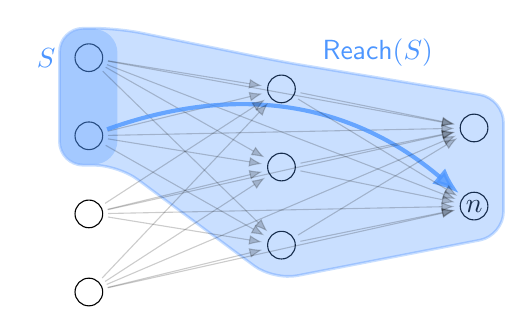
\begin{tikzpicture}[loose/.style={inner sep=.7em},edge/.style = {->,-Latex},
    oval/.style={ellipse,draw}]
    
        %--------------------------------------------
        % Nodes
        \node[circle,minimum size=10pt,inner sep=0pt,outer sep=2pt,fill=white,draw](a){};
        \node[below=0.5 of a,circle,minimum size=10pt,inner sep=0pt,outer sep=2pt,fill=white,draw](b){};
        \node[below=0.5 of b,circle,minimum size=10pt,inner sep=0pt,outer sep=2pt,fill=white,draw](c){};
        \node[below=0.5 of c,circle,minimum size=10pt,inner sep=0pt,outer sep=2pt,fill=white,draw](d){};
        % \node[below=0.5 of d,circle,minimum size=10pt,inner sep=0pt,outer sep=2pt,fill=white,draw](e){};
        \node[right=2.2 of $(a)!0.2!(c)$,circle,minimum size=10pt,inner sep=0pt,outer sep=2pt,fill=white,draw](f){};
        \node[below=0.5 of f,circle,minimum size=10pt,inner sep=0pt,outer sep=2pt,fill=white,draw](g){};
        \node[below=0.5 of g,circle,minimum size=10pt,inner sep=0pt,outer sep=2pt,fill=white,draw](h){};
        % \node[below=0.5 of h,circle,minimum size=10pt,inner sep=0pt,outer sep=2pt,fill=white,draw](i){};
        \node[right=2.2 of $(f)!0.5!(g)$,circle,minimum size=10pt,inner sep=0pt,outer sep=2pt,fill=white,draw](j){};
        \node[below=0.5 of j,circle,minimum size=10pt,inner sep=0pt,outer sep=2pt,fill=white,draw](k){$n$};
        % \node[below=0.5 of k,circle,minimum size=10pt,inner sep=0pt,outer sep=2pt,fill=white,draw](l){};
        % Hidden nodes
        
        %--------------------------------------------
        % The set S
        \node[fill=myblue, color=myblue, very thick, opacity=0.3,rectangle,rounded corners=2ex,fit=(a) (b)]{};
        
        %--------------------------------------------
        % The propagation of S
        \begin{scope}[transparency group]
        \begin{scope}[blend mode=multiply]
        \draw[fill=myblue, color=myblue, opacity=0.3, rounded corners=2ex] 
                ([xshift=-0.2cm,yshift=0.2cm] a.north west)
            -- ([xshift=0.2cm,yshift=0.2cm] a.north east)
            -- ([yshift=0.10cm] f.north)
            % -- ([xshift=-0.2cm,yshift=0.2cm] j.north west)
            -- ([xshift=0.2cm,yshift=0.2cm] j.north east)
            
            -- ([xshift=0.2cm,yshift=-0.2cm] k.south east)
            % -- ([xshift=-0.2cm,yshift=-0.2cm] k.south west)
            -- ([xshift=-0.1cm,yshift=-0.2cm] h.south)
            -- ([xshift=0.2cm,yshift=-0.2cm] b.south east)
            -- ([xshift=-0.2cm,yshift=-0.2cm] b.south west)
            -- cycle;
        \end{scope}
        \end{scope}

        %--------------------------------------------
        % Set Labels
        \node [color=myblue,opacity=1,left=0.3 of $(a)$]{$S$};
        \node [color=myblue,opacity=1, above=0.9 of $(g)!0.5!(j)$]{$\Reach(S)$};
        
        %--------------------------------------------
        % Edges
        \draw[edge, color=black, opacity=0.2] (a) -- (f) node [near start, above] {};
        \draw[edge, color=black, opacity=0.2] (a) -- (h) node [near start, above] {};
        % \draw[edge, color=black, opacity=0.2] (a) -- (i) node [near start, above] {};
        \draw[edge, color=black, opacity=0.2] (a) -- (g) node [near start, above] {};
        \draw[edge, color=black, opacity=0.2] (a) -- (j) node [near start, above] {};
        \draw[edge, color=black, opacity=0.2] (a) -- (k) node [near start, above] {};
        % \draw[edge, color=black, opacity=0.2] (a) -- (l) node [near start, above] {};
        \draw[edge, color=black, opacity=0.2] (b) -- (f) node [below=-0.1, near start] {};
        \draw[edge, color=black, opacity=0.2] (b) -- (g) node [near start, above=-0.15] {};
        \draw[edge, color=black, opacity=0.2] (b) -- (h) node [below=-0.1, near start] {};
        % \draw[edge, color=black, opacity=0.2] (b) -- (i) node [below=-0.1, near start] {};
        \draw[edge, color=black, opacity=0.2] (b) -- (j) node [below=-0.1, near start] {};
        \draw[edge, line width=1.5pt, color=myblue, opacity=0.8] (b) to [bend left] (k);
        % \draw[edge, line width=1.5pt, color=myblue, opacity=0.8] (b) -- (k) node [below=-0.1, near start] {};
        % \draw[edge, color=black, opacity=0.2] (b) -- (l) node [below=-0.1, near start] {};
        \draw[edge, color=black, opacity=0.2] (c) -- (f) node [near start, below=-0.1] {};
        \draw[edge, color=black, opacity=0.2] (c) -- (g) node [near start, above=-0.1] {};
        \draw[edge, color=black, opacity=0.2] (c) -- (h) node [near start, above=-0.1] {};
        % \draw[edge, color=black, opacity=0.2] (c) -- (i) node [near start, above=-0.1] {};
        \draw[edge, color=black, opacity=0.2] (c) -- (j) node [near start, above=-0.1] {};
        \draw[edge, color=black, opacity=0.2] (c) -- (k) node [near start, above=-0.1] {};
        % \draw[edge, color=black, opacity=0.2] (c) -- (l) node [near start, above=-0.1] {};
        \draw[edge, color=black, opacity=0.2] (d) -- (f) node [near start, below=-0.1] {};
        \draw[edge, color=black, opacity=0.2] (d) -- (g) node [near start, above=-0.1] {};
        \draw[edge, color=black, opacity=0.2] (d) -- (h) node [near start, above=-0.1] {};
        % \draw[edge, color=black, opacity=0.2] (d) -- (i) node [near start, above=-0.1] {};
        \draw[edge, color=black, opacity=0.2] (d) -- (j) node [near start, above=-0.1] {};
        \draw[edge, color=black, opacity=0.2] (d) -- (k) node [near start, above=-0.1] {};
        % \draw[edge, color=black, opacity=0.2] (d) -- (l) node [near start, above=-0.1] {};
        % \draw[edge, color=black, opacity=0.2] (e) -- (f) node [near start, below] {};
        % \draw[edge, color=black, opacity=0.2] (e) -- (g) node [near start, below] {};
        % \draw[edge, color=black, opacity=0.2] (e) -- (h) node [near start, below] {};
        % \draw[edge, color=black, opacity=0.2] (e) -- (i) node [near start, below] {};
        % \draw[edge, color=black, opacity=0.2] (e) -- (j) node [near start, below] {};
        % \draw[edge, color=black, opacity=0.2] (e) -- (k) node [near start, below] {};
        % \draw[edge, color=black, opacity=0.2] (e) -- (l) node [near start, below] {};
        \draw[edge, color=black, opacity=0.2] (f) -- (j) node [near start, below] {};
        \draw[edge, color=black, opacity=0.2] (f) -- (k) node [near start, below] {};
        % \draw[edge, color=black, opacity=0.2] (f) -- (l) node [near start, below] {};
        \draw[edge, color=black, opacity=0.2] (g) -- (j) node [near start, below] {};
        \draw[edge, color=black, opacity=0.2] (g) -- (k) node [near start, below] {};
        % \draw[edge, color=black, opacity=0.2] (g) -- (l) node [near start, below] {};
        \draw[edge, color=black, opacity=0.2] (h) -- (j) node [near start, below] {};
        \draw[edge, color=black, opacity=0.2] (h) -- (k) node [near start, below] {};
        % \draw[edge, color=black, opacity=0.2] (h) -- (l) node [near start, below] {};
        % \draw[edge, color=black, opacity=0.2] (i) -- (j) node [near start, below] {};
        % \draw[edge, color=black, opacity=0.2] (i) -- (k) node [near start, below] {};
        % \draw[edge, color=black, opacity=0.2] (i) -- (l) node [near start, below] {};
    \end{tikzpicture}
    \caption{The graph reachability operator $\Reach$.}
    \label{fig:reachable}
\end{figure}

The $\Reach$ operator is just ordinary graph-reachability: $\Reach(S)$ returns the set of all neurons reachable from $S$ (illustrated in Figure~\ref{fig:reachable}).  Formally, $\Reach_\Net : \State \to \State$ is given by $n \in \Reach(S)$ iff there exists $m \in S$ with an $E$-path from $m$ to $n$.

$\Reach$ is not a very interesting operator in its own right, but we include it because graph reachability is necessary for reasoning about Hebbian learning. It's easy to check that $\Reach$ is an ordinary monotonic closure operator.  Moreover, $\Reach$ is closed under union.
\begin{restatable}{proposition}{reachproperties}
% \begin{proposition}\label{reach-properties}
    \label{reach-properties}
    For all $S, A, B \in \State$,
    \begin{description}
        \item[Inclusion.] $S \subseteq \Reach(S)$
        \item[Idempotent.] $\Reach(\Reach(S)) = \Reach(S)$
        \item[Monotonic.] If $A \subseteq B$ then $\Reach(A) \subseteq \Reach(B)$.
        \item[Closed under $\cup$.] $\Reach(A \cup B) = \Reach(A) \cup \Reach(B)$
    \end{description}
\end{restatable}
% Proposition~\ref{reach-properties} characterizes $\Reach$ as an ordinary monotonic closure operator. Think of $\Reach$ as the monotonic counterpart to $\Prop$.  $\Reach$ is not a very interesting operator in its own right, but we include it because graph reachability is necessary for reasoning about Hebbian learning.

The more important operator is $\Prop$, which captures how activation patterns are ``propagated forward'' through the net.  As we mentioned in the Introduction, the idea is that active neurons in a state $S$ successively activate new neurons.  The activation of each neuron $n$ is a function of its predecessor's activations.  $\Prop(S)$ returns the state at the fixed point of the process, i.e., the set of all neurons that are eventually activated on input $S$ (illustrated in Figure~\ref{fig:propagate}).

We formalize forward propagation as follows, drawing heavily from~\cite{leitgeb2001nonmonotonic}.
\begin{definition}
    Let $n \in N$, and let $\vec{m} = m_1, \ldots, m_{\degree{n}}$ list the predecessors of $n$.  We define $\Prop_\Net : \State \to \State$ recursively on $l = \layer{n}$ as follows.
    \begin{description}
        \item[Base ($l=0$).] $n \in \Prop_\Net(S)$ iff $n \in S$
        \item[Constructor ($l\geq0$).] $n \in \Prop_\Net(S)$ iff either $n \in S$, or $n$ is activated by its predecessors $m_i \in \Prop_\Net(S)$, i.e.,
        \[
            A(\sum_{i=1}^{\degree{n}} W(m_i, n) \cdot \bigchi_{\Prop_\Net(S)}(m_i)) = 1
        \]
    \end{description}
    If $\Net$ is clear from context, we just write $\Prop(S)$.
\end{definition}
Note that $\Prop$ is well-founded, since all predecessors $m_i \in \preds{n}$ have $\layer{m_i} < \layer{n}$.  Also note that our definition differs somewhat from~\cite{leitgeb2001nonmonotonic}, which defines $\Prop$ over \emph{inhibition nets} --- weightless nets with both excitatory and inhibitory connections.  But that paper also proves that inhibition nets and binary, feed-forward nets have the same $\Prop$-structure.  So we import the results here.

\begin{figure}
    \centering
    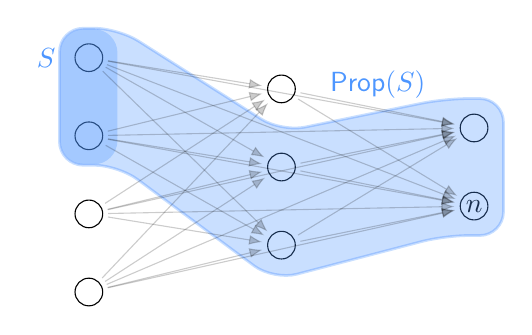
\begin{tikzpicture}[loose/.style={inner sep=.7em},edge/.style = {->,-Latex},
    oval/.style={ellipse,draw}]
    
        %--------------------------------------------
        % Nodes
        \node[circle,minimum size=10pt,inner sep=0pt,outer sep=2pt,fill=white,draw](a){};
        \node[below=0.5 of a,circle,minimum size=10pt,inner sep=0pt,outer sep=2pt,fill=white,draw](b){};
        \node[below=0.5 of b,circle,minimum size=10pt,inner sep=0pt,outer sep=2pt,fill=white,draw](c){};
        \node[below=0.5 of c,circle,minimum size=10pt,inner sep=0pt,outer sep=2pt,fill=white,draw](d){};
        % \node[below=0.5 of d,circle,minimum size=10pt,inner sep=0pt,outer sep=2pt,fill=white,draw](e){};
        \node[right=2.2 of $(a)!0.2!(c)$,circle,minimum size=10pt,inner sep=0pt,outer sep=2pt,fill=white,draw](f){};
        \node[below=0.5 of f,circle,minimum size=10pt,inner sep=0pt,outer sep=2pt,fill=white,draw](g){};
        \node[below=0.5 of g,circle,minimum size=10pt,inner sep=0pt,outer sep=2pt,fill=white,draw](h){};
        % \node[below=0.5 of h,circle,minimum size=10pt,inner sep=0pt,outer sep=2pt,fill=white,draw](i){};
        \node[right=2.2 of $(f)!0.5!(g)$,circle,minimum size=10pt,inner sep=0pt,outer sep=2pt,fill=white,draw](j){};
        \node[below=0.5 of j,circle,minimum size=10pt,inner sep=0pt,outer sep=2pt,fill=white,draw](k){$n$};
        % \node[below=0.5 of k,circle,minimum size=10pt,inner sep=0pt,outer sep=2pt,fill=white,draw](l){};
        % Hidden nodes
        
        %--------------------------------------------
        % The set S
        \node[fill=myblue, color=myblue, very thick, opacity=0.3,rectangle,rounded corners=2ex,fit=(a) (b)]{};
        
        %--------------------------------------------
        % The propagation of S
        \begin{scope}[transparency group]
        \begin{scope}[blend mode=multiply]
        \draw[fill=myblue, color=myblue, opacity=0.3, rounded corners=2ex] 
               ([xshift=-0.2cm,yshift=0.2cm] a.north west)
            -- ([xshift=0.2cm,yshift=0.2cm] a.north east)
            -- ([yshift=0.2cm] g.north)
            -- ([xshift=-0.2cm,yshift=0.2cm] j.north west)
            -- ([xshift=0.2cm,yshift=0.2cm] j.north east)
            
            -- ([xshift=0.2cm,yshift=-0.2cm] k.south east)
            -- ([xshift=-0.2cm,yshift=-0.2cm] k.south west)
            -- ([xshift=-0.1cm,yshift=-0.2cm] h.south)
            -- ([xshift=0.2cm,yshift=-0.2cm] b.south east)
            -- ([xshift=-0.2cm,yshift=-0.2cm] b.south west)
            -- cycle;
        \end{scope}
        \end{scope}
         
        %--------------------------------------------
        % Set Labels
        \node [color=myblue,opacity=1,left=0.3 of $(a)$]{$S$};
        \node [color=myblue,opacity=1, above=0.5 of $(g)!0.5!(j)$]{$\Prop(S)$};
        
        %--------------------------------------------
        % Edges
        \draw[edge, color=black, opacity=0.2] (a) -- (f) node [near start, above] {};
        \draw[edge, color=black, opacity=0.2] (a) -- (h) node [near start, above] {};
        % \draw[edge, color=black, opacity=0.2] (a) -- (i) node [near start, above] {};
        \draw[edge, color=black, opacity=0.2] (a) -- (g) node [near start, above] {};
        \draw[edge, color=black, opacity=0.2] (a) -- (j) node [near start, above] {};
        \draw[edge, color=black, opacity=0.2] (a) -- (k) node [near start, above] {};
        % \draw[edge, color=black, opacity=0.2] (a) -- (l) node [near start, above] {};
        \draw[edge, color=black, opacity=0.2] (b) -- (f) node [below=-0.1, near start] {};
        \draw[edge, color=black, opacity=0.2] (b) -- (g) node [near start, above=-0.15] {};
        \draw[edge, color=black, opacity=0.2] (b) -- (h) node [below=-0.1, near start] {};
        % \draw[edge, color=black, opacity=0.2] (b) -- (i) node [below=-0.1, near start] {};
        \draw[edge, color=black, opacity=0.2] (b) -- (j) node [below=-0.1, near start] {};
        \draw[edge, color=black, opacity=0.2] (b) -- (k) node [below=-0.1, near start] {};
        % \draw[edge, color=black, opacity=0.2] (b) -- (l) node [below=-0.1, near start] {};
        \draw[edge, color=black, opacity=0.2] (c) -- (f) node [near start, below=-0.1] {};
        \draw[edge, color=black, opacity=0.2] (c) -- (g) node [near start, above=-0.1] {};
        \draw[edge, color=black, opacity=0.2] (c) -- (h) node [near start, above=-0.1] {};
        % \draw[edge, color=black, opacity=0.2] (c) -- (i) node [near start, above=-0.1] {};
        \draw[edge, color=black, opacity=0.2] (c) -- (j) node [near start, above=-0.1] {};
        \draw[edge, color=black, opacity=0.2] (c) -- (k) node [near start, above=-0.1] {};
        % \draw[edge, color=black, opacity=0.2] (c) -- (l) node [near start, above=-0.1] {};
        \draw[edge, color=black, opacity=0.2] (d) -- (f) node [near start, below=-0.1] {};
        \draw[edge, color=black, opacity=0.2] (d) -- (g) node [near start, above=-0.1] {};
        \draw[edge, color=black, opacity=0.2] (d) -- (h) node [near start, above=-0.1] {};
        % \draw[edge, color=black, opacity=0.2] (d) -- (i) node [near start, above=-0.1] {};
        \draw[edge, color=black, opacity=0.2] (d) -- (j) node [near start, above=-0.1] {};
        \draw[edge, color=black, opacity=0.2] (d) -- (k) node [near start, above=-0.1] {};
        % \draw[edge, color=black, opacity=0.2] (d) -- (l) node [near start, above=-0.1] {};
        % \draw[edge, color=black, opacity=0.2] (e) -- (f) node [near start, below] {};
        % \draw[edge, color=black, opacity=0.2] (e) -- (g) node [near start, below] {};
        % \draw[edge, color=black, opacity=0.2] (e) -- (h) node [near start, below] {};
        % \draw[edge, color=black, opacity=0.2] (e) -- (i) node [near start, below] {};
        % \draw[edge, color=black, opacity=0.2] (e) -- (j) node [near start, below] {};
        % \draw[edge, color=black, opacity=0.2] (e) -- (k) node [near start, below] {};
        % \draw[edge, color=black, opacity=0.2] (e) -- (l) node [near start, below] {};
        \draw[edge, color=black, opacity=0.2] (f) -- (j) node [near start, below] {};
        \draw[edge, color=black, opacity=0.2] (f) -- (k) node [near start, below] {};
        % \draw[edge, color=black, opacity=0.2] (f) -- (l) node [near start, below] {};
        \draw[edge, color=black, opacity=0.2] (g) -- (j) node [near start, below] {};
        \draw[edge, color=black, opacity=0.2] (g) -- (k) node [near start, below] {};
        % \draw[edge, color=black, opacity=0.2] (g) -- (l) node [near start, below] {};
        \draw[edge, color=black, opacity=0.2] (h) -- (j) node [near start, below] {};
        \draw[edge, color=black, opacity=0.2] (h) -- (k) node [near start, below] {};
        % \draw[edge, color=black, opacity=0.2] (h) -- (l) node [near start, below] {};
        % \draw[edge, color=black, opacity=0.2] (i) -- (j) node [near start, below] {};
        % \draw[edge, color=black, opacity=0.2] (i) -- (k) node [near start, below] {};
        % \draw[edge, color=black, opacity=0.2] (i) -- (l) node [near start, below] {};
    \end{tikzpicture}
    \caption{The forward propagation operator $\Prop$.}
    \label{fig:propagate}
\end{figure}

We can think of $\Prop$ as the nonmonotonic counterpart to $\Reach$; it is not the case that for all $A, B \in \State$, if $A \subseteq B$ then $\Prop(A) \subseteq \Prop(B)$.  This is because our net's weights can be negative, and so $\Prop(B)$ can inhibit the activation of new neurons that would otherwise be activated by $\Prop(A)$.  Instead, we can characterize $\Prop$ as a loop-cumulative closure operator.
\begin{restatable}{proposition}{propagationproperties}\cite{leitgeb2001nonmonotonic}\label{propagation-properties}
    Let $S, S_1, \ldots, S_k \in \State$.
    \begin{description}
        \item[Inclusion.] $S \subseteq \Prop(S)$
        \item[Idempotence.] $\Prop(\Prop(S)) = \Prop(S)$
        \item[Cumulative.] If $S_1 \subseteq S_2 \subseteq \Prop(S_1)$,\\ then $\Prop(S_1) = \Prop(S_2)$
        \item[Loop.] If $S_1 \subseteq \Prop(S_0), \ldots, S_k \subseteq \Prop(S_{k-1})$, and $S_0 \subseteq \Prop(S_k)$, then $\Prop(S_i) = \Prop(S_j)$ for all $i, j \in \set{0, \ldots, k}$
    \end{description}
\end{restatable}
These Loop and Cumulative properties together are a well-known weakening of monotonicity (see~\cite{kraus1990nonmonotonic}).

%-------------------------------------------
\subsection{Syntax, Semantics, and Base Axioms}

Now let us state formally the specific logic and neural network semantics we consider.  Let $p, q, \ldots$ be finitely many atomic variables. These represent fixed states, corresponding to features in the external world that we know ahead of time.  Usually these are input and output states, although they could be intermediate ``hidden'' states if we know these features ahead of time.  For example, $p$ might be the set of neurons that represent the color \emph{pink}.  For more complex formulas,
\begin{definition}
    Formulas of our language $\uplang$ are given by
    \[
        \varphi, \psi ::= p \mid \neg \varphi \mid \varphi \land \psi \mid \Know{\varphi} \mid \Typ{\varphi} \mid \Hebbop{\varphi} \psi
    \]
    We define $\top, \bot, \lor, \to, \leftrightarrow$, and the dual modal operators $\diaKnow, \diaTyp, \diaHebbop{\varphi}$ in the usual way.  Additionally, let our base language $\lang$ consist of all the $\Hebbop{\varphi}$-free formulas in $\uplang$.
\end{definition}

First, let us give intuitive readings for these formulas; we will soon ground these readings with formal semantics.  $\Know{\varphi}$ reads ``the agent \emph{knows} $\varphi$,'' and $\Typ{\varphi}$ reads ``the \emph{typical} $\varphi$'' or sententially as ``\emph{typically} $\varphi$.'' Note that we can express conditionals $\varphi \Rightarrow \psi$ in this language as $\Typ{\varphi} \to \psi$, i.e., ``the typical $\varphi$ is $\psi$.''  Finally, the dynamic operator $\Hebbop{\varphi} \psi$ reads ``after the agent learns $\varphi$, $\psi$ holds.''  In Section~6, we will discuss the sense in which this learning is a plausibility upgrade.

% For the rest of this section, we focus on the base logic (over $\lang$).  A model for this logic is just a net $\Net \in \AllNets$ along with an interpretation function $\semantics{\cdot}_\Net : \lang \to \State$. We drop the subscript when $\Net$ is clear from context.  The idea for $\semantics{\cdot}_\Net$ is simply to map $\diaKnowNoArgs$ to $\Reach$ and $\diaTypNoArgs$ to $\Prop$.

Formally, a model for this logic is just a net $\Net \in \AllNets$ along with an interpretation function $\semantics{\cdot}_\Net : \lang \to \State$ that maps each formula to the set of neurons it denotes. We drop the subscript when $\Net$ is clear from context.  For the base logic formulas (over $\lang$), the idea is to map possible knowledge $\diaKnowNoArgs$ to $\Reach$ and possible typicality $\diaTypNoArgs$ to $\Prop$.  In the next section, we will explain how we map $\Hebbop{\varphi}$ to Hebbian learning.
\begin{definition}
    The semantics of our base logic is given recursively, using the dual forms $\diaKnowNoArgs$ and $\diaTypNoArgs$, as follows.
    \[
    \begin{array}{lcl}
        \semantics{p} & \in &  \State \mbox{ is fixed, nonempty} \\
        \semantics{\neg \varphi} & = & \semantics{\varphi}^\complement \\
        \semantics{\varphi \land \psi} & = & \semantics{\varphi} \cap \semantics{\psi} \\
        \semantics{\diaKnow{\varphi}} & = & \Reach(\semantics{\varphi}) \\
        \semantics{\diaTyp{\varphi}} & = & \Prop(\semantics{\varphi})
    \end{array}
    \]
\end{definition}
To better understand this mapping, think of the net $\Net$ loosely as a kind of possible worlds model.  Its edges represent epistemic accessibility; the nodes reachable from $\semantics{\varphi}$ are the nodes where it's \emph{possible to know} $\varphi$.  Similarly, the propagation of $\semantics{\varphi}$, determined by the weights of the net, constrains which nodes it is \emph{possible to find typical} of $\varphi$.  In this sense, the propagation $\Prop(\semantics{\varphi})$ is dual to the notion of a \emph{prototype} in psychology~\cite{murphy2004big}.

So far, we have defined formulas in terms of the features they denote, e.g., the color \emph{pink}.  But we can also read formulas sententially, e.g., ``the current state is pink.''  We consider the sentence $\varphi$ to be \emph{true} in a net $\Net$ as follows.
\begin{definition}
    $\Net \models \varphi$ iff $\semantics{\varphi}_\Net = N$
\end{definition}
An important special case is the conditional $\varphi \Rightarrow \psi$.  As before, we express this (over $\lang$) as $\Typ{\varphi} \to \psi$.  Observe that this is true whenever $\Prop(\semantics{\varphi}) \supseteq \semantics{\psi}$, which tells us whether, given input $\semantics{\varphi}$, the net's propagated state includes $\semantics{\psi}$.  So $\varphi \Rightarrow \psi$ conveniently expresses ``the net \emph{classifies} $\varphi$ as $\psi$.''

We define the logic's proof system in the usual way (the following applies to both $\lang$ and $\uplang$).  We have $\proves \varphi$ iff either $\varphi$ is an axiom, or $\varphi$ follows from previously obtained formulas by one of the inference rules.  For a set of formulas $\Gamma$, $\Gamma \proves \varphi$ holds if there exist finitely many $\psi_1, \ldots, \psi_k \in \Gamma$ such that $\proves \psi_1 \land \cdots \land \psi_k \to \varphi$.  A set $\Gamma$ is consistent if $\Gamma \not \proves \bot$.

We now list axioms for the base logic.  We should emphasize that these axioms may not be complete, and we leave this question to future work.  Rather, our focus in this paper is on the completeness of the dynamic operator $\Hebbop{\varphi}$, \emph{given} the completeness of the base logic.

For $\TypNoArgs$ alone,~\cite{leitgeb2001nonmonotonic} proves that the properties in Proposition~\ref{propagation-properties} are complete for $\Prop$ over binary, feed-forward nets.  We transcribe these into our modal language.
\begin{description}
    \item[Nec.] From $\proves \varphi$ we can infer $\proves \Typ{\varphi}$
    \item[Dual.] $\diaTyp{\varphi} \leftrightarrow \neg \Typ{\neg \varphi}$
    \item[Refl.] $\Typ{\varphi} \to \varphi$
    \item[Trans.] $\Typ{\varphi} \to \Typ{\Typ{\varphi}}$
    \item[Cumulative.] $(\varphi \to \psi) \land (\Typ{\psi} \to \varphi) \to (\Typ{\varphi} \to \psi)$
    \item[Loop.] $(\Typ \varphi_0 \to \varphi_1) \land \cdots \land (\Typ \varphi_k \to \varphi_0)\\ 
    \hspace*{3em} \to (\Typ \varphi_0 \to \varphi_k)$
\end{description}
But remember that our nets are also fully connected!  So we need to modify the model construction from~\cite{leitgeb2001nonmonotonic} by introducing a zero weight edge between every pair of previously unconnected nodes.  Note that this change does not affect the $\Prop$-structure of the net.

As for $\KnowNoArgs$, we at least have the following sound axioms, transcribed from Proposition~\ref{reach-properties}.
\begin{description}
    \item[Nec.] From $\proves \varphi$ we can infer $\proves \Know{\varphi}$
    \item[Dual.] $\diaKnow{\varphi} \leftrightarrow \neg \Know{\neg \varphi}$
    \item[Distr.] $\Know{(\varphi \to \psi)} \leftrightarrow (\Know{\varphi} \to \Know{\psi})$
    \item[Refl.] $\Know{\varphi} \to \varphi$
    \item[Trans.] $\Know{\varphi} \to \Know{\Know{\varphi}}$
\end{description}
These axioms are the usual complete axioms for normal modal logic over reflexive and transitive frames.  So far these axioms seem innocuous enough.  But for completeness, the catch is that $\KnowNoArgs$ and $\TypNoArgs$ may interact in ways that affect the model construction.  For example, the following axiom is easy to check, but it is not clear whether it is sufficient.
\begin{description}
    \item[Incl.] $\Know{\varphi} \to \Typ{\varphi}$
\end{description}

%═══════════════════════════════════════════
% 4. The Dynamics of \hebb{\varphi}
%═══════════════════════════════════════════
\section{Dynamics of Iterated Hebbian Update}

%-------------------------------------------
\subsection{Single-Step Hebbian Update}

The plan from here is to extend this base logic with a dynamic operator $\Hebbop{\varphi}$ for Hebbian update.  Hebb's classic learning rule~\cite{hebb-organization-of-behavior-1949} states that when two adjacent neurons are simultaneously and persistently active, the connection between them strengthens.  In contrast with, e.g., backpropagation, Hebbian learning is errorless and unsupervised. Another key difference is that Hebbian update is local --- the change in a weight $\Delta W(m, n)$ depends only on the activation of the immediately adjacent neurons. For this reason, the Hebbian family of learning policies is often considered more biologically plausible than backpropagation. There are many variations of Hebbian learning, but we only consider the most basic form of Hebb's rule: $\Delta W(m, n) = \eta x_m x_n$, where $\eta$ is the learning rate and $x_m, x_n$ are the outputs of adjacent neurons $m$ and $n$.  Note that this is the \emph{unstable} variation of Hebb's rule; repeatedly applying the rule will make the weights arbitrarily large.  In this paper, we will not consider stabilizing variants such as Oja's rule~\cite{oja1982simplified}.

Before we formalize iterated Hebbian learning, let us consider a single step of Hebbian update $\HebbNoArgs$.  Given a net $\Net$ and a state $S$, we first forward-propagate $S$ through $\Net$.  Intuitively, $\Hebb{\Net}{S}$ returns the net that we obtain by applying Hebb's rule: Any edges that are involved in the propagated activation pattern simply have their weights strengthened.  This is illustrated in Figure~\ref{fig:hebbian-update}.

% Our goal is to model iterated Hebbian update $\HebbstarNoArgs$ as the fixed-point of repeatedly applying Hebb's rule.  But first, we define a function $\HebbNoArgs$ for \emph{single-step update}.  $\Hebb{\Net}{S}$ strengthens those edges in a net $\Net \in \AllNets$ whose neurons are active when we feed $\Net$ a signal $S \in \State$. (Both $\HebbNoArgs$ and $\HebbstarNoArgs$ are illustrated in Figure~\ref{fig:hebbian-update}.)

\begin{figure}
    \centering
    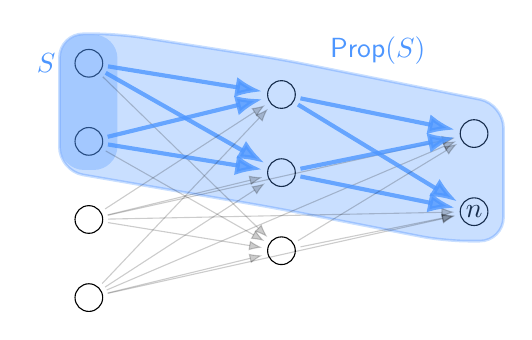
\begin{tikzpicture}[loose/.style={inner sep=.7em},edge/.style = {->,-Latex},
    oval/.style={ellipse,draw}]
    
        %--------------------------------------------
        % Nodes
        \node[circle,minimum size=10pt,inner sep=0pt,outer sep=2pt,fill=white,draw](a){};
        \node[below=0.5 of a,circle,minimum size=10pt,inner sep=0pt,outer sep=2pt,fill=white,draw](b){};
        \node[below=0.5 of b,circle,minimum size=10pt,inner sep=0pt,outer sep=2pt,fill=white,draw](c){};
        \node[below=0.5 of c,circle,minimum size=10pt,inner sep=0pt,outer sep=2pt,fill=white,draw](d){};
        % \node[below=0.5 of d,circle,minimum size=10pt,inner sep=0pt,outer sep=2pt,fill=white,draw](e){};
        \node[right=2.2 of $(a)!0.2!(c)$,circle,minimum size=10pt,inner sep=0pt,outer sep=2pt,fill=white,draw](f){};
        \node[below=0.5 of f,circle,minimum size=10pt,inner sep=0pt,outer sep=2pt,fill=white,draw](g){};
        \node[below=0.5 of g,circle,minimum size=10pt,inner sep=0pt,outer sep=2pt,fill=white,draw](h){};
        % \node[below=0.5 of h,circle,minimum size=10pt,inner sep=0pt,outer sep=2pt,fill=white,draw](i){};
        \node[right=2.2 of $(f)!0.5!(g)$,circle,minimum size=10pt,inner sep=0pt,outer sep=2pt,fill=white,draw](j){};
        \node[below=0.5 of j,circle,minimum size=10pt,inner sep=0pt,outer sep=2pt,fill=white,draw](k){$n$};
        % \node[below=0.5 of k,circle,minimum size=10pt,inner sep=0pt,outer sep=2pt,fill=white,draw](l){};
        % Hidden nodes
        
        %--------------------------------------------
        % The set S
        \node[fill=myblue, color=myblue, very thick, opacity=0.3,rectangle,rounded corners=2ex,fit=(a) (b)]{};
        
        %--------------------------------------------
        % The propagation of S
        \begin{scope}[transparency group]
        \begin{scope}[blend mode=multiply]
        \draw[fill=myblue, color=myblue, opacity=0.3, rounded corners=2ex] 
               ([xshift=-0.2cm,yshift=0.2cm] a.north west)
            -- ([xshift=0.2cm,yshift=0.2cm] a.north east)
            -- ([yshift=0.2cm] f.north)
            % -- ([xshift=-0.2cm,yshift=0.2cm] j.north west)
            -- ([xshift=0.2cm,yshift=0.2cm] j.north east)
            
            -- ([xshift=0.2cm,yshift=-0.2cm] k.south east)
            -- ([xshift=-0.2cm,yshift=-0.2cm] k.south west)
            -- ([xshift=-0.1cm,yshift=-0.2cm] g.south)
            % -- ([xshift=0.2cm,yshift=-0.2cm] b.south east)
            -- ([xshift=-0.2cm,yshift=-0.2cm] b.south west)
            -- cycle;
        \end{scope}
        \end{scope}
         
        %--------------------------------------------
        % Set Labels
        \node [color=myblue,opacity=1,left=0.3 of $(a)$]{$S$};
        \node [color=myblue,opacity=1, above=1.0 of $(g)!0.5!(j)$]{$\Prop(S)$};
        
        %--------------------------------------------
        % Edges
        % \draw[edge, color=black, opacity=0.2] (a) -- (f) node [near start, above] {};
        \draw[edge, line width=1.5pt, color=myblue, opacity=0.8] (a) to (f);
        \draw[edge, color=black, opacity=0.2] (a) -- (h) node [near start, above] {};
        % \draw[edge, color=black, opacity=0.2] (a) -- (i) node [near start, above] {};
        % \draw[edge, color=black, opacity=0.2] (a) -- (g) node [near start, above] {};
        \draw[edge, line width=1.5pt, color=myblue, opacity=0.8] (a) to (g);
        % \draw[edge, color=black, opacity=0.2] (a) -- (j) node [near start, above] {};
        % \draw[edge, color=black, opacity=0.2] (a) -- (k) node [near start, above] {};
        % \draw[edge, color=black, opacity=0.2] (a) -- (l) node [near start, above] {};
        % \draw[edge, color=black, opacity=0.2] (b) -- (f) node [below=-0.1, near start] {};
        \draw[edge, line width=1.5pt, color=myblue, opacity=0.8] (b) to (f);
        % \draw[edge, color=black, opacity=0.2] (b) -- (g) node [near start, above=-0.15] {};
        \draw[edge, line width=1.5pt, color=myblue, opacity=0.8] (b) to (g);
        \draw[edge, color=black, opacity=0.2] (b) -- (h) node [below=-0.1, near start] {};
        % \draw[edge, color=black, opacity=0.2] (b) -- (i) node [below=-0.1, near start] {};
        % \draw[edge, color=black, opacity=0.2] (b) -- (j) node [below=-0.1, near start] {};
        % \draw[edge, color=black, opacity=0.2] (b) -- (k) node [below=-0.1, near start] {};
        % \draw[edge, color=black, opacity=0.2] (b) -- (l) node [below=-0.1, near start] {};
        \draw[edge, color=black, opacity=0.2] (c) -- (f) node [near start, below=-0.1] {};
        \draw[edge, color=black, opacity=0.2] (c) -- (g) node [near start, above=-0.1] {};
        \draw[edge, color=black, opacity=0.2] (c) -- (h) node [near start, above=-0.1] {};
        % \draw[edge, color=black, opacity=0.2] (c) -- (i) node [near start, above=-0.1] {};
        \draw[edge, color=black, opacity=0.2] (c) -- (j) node [near start, above=-0.1] {};
        \draw[edge, color=black, opacity=0.2] (c) -- (k) node [near start, above=-0.1] {};
        % \draw[edge, color=black, opacity=0.2] (c) -- (l) node [near start, above=-0.1] {};
        \draw[edge, color=black, opacity=0.2] (d) -- (f) node [near start, below=-0.1] {};
        \draw[edge, color=black, opacity=0.2] (d) -- (g) node [near start, above=-0.1] {};
        \draw[edge, color=black, opacity=0.2] (d) -- (h) node [near start, above=-0.1] {};
        % \draw[edge, color=black, opacity=0.2] (d) -- (i) node [near start, above=-0.1] {};
        \draw[edge, color=black, opacity=0.2] (d) -- (j) node [near start, above=-0.1] {};
        \draw[edge, color=black, opacity=0.2] (d) -- (k) node [near start, above=-0.1] {};
        % \draw[edge, color=black, opacity=0.2] (d) -- (l) node [near start, above=-0.1] {};
        % \draw[edge, color=black, opacity=0.2] (e) -- (f) node [near start, below] {};
        % \draw[edge, color=black, opacity=0.2] (e) -- (g) node [near start, below] {};
        % \draw[edge, color=black, opacity=0.2] (e) -- (h) node [near start, below] {};
        % \draw[edge, color=black, opacity=0.2] (e) -- (i) node [near start, below] {};
        % \draw[edge, color=black, opacity=0.2] (e) -- (j) node [near start, below] {};
        % \draw[edge, color=black, opacity=0.2] (e) -- (k) node [near start, below] {};
        % \draw[edge, color=black, opacity=0.2] (e) -- (l) node [near start, below] {};
        % \draw[edge, color=black, opacity=0.2] (f) -- (j) node [near start, below] {};
        \draw[edge, line width=1.5pt, color=myblue, opacity=0.8] (f) to (j);
        % \draw[edge, color=black, opacity=0.2] (f) -- (k) node [near start, below] {};
        \draw[edge, line width=1.5pt, color=myblue, opacity=0.8] (f) to (k);
        % \draw[edge, color=black, opacity=0.2] (f) -- (l) node [near start, below] {};
        % \draw[edge, color=black, opacity=0.2] (g) -- (j) node [near start, below] {};
        \draw[edge, line width=1.5pt, color=myblue, opacity=0.8] (g) to (j);
        % \draw[edge, color=black, opacity=0.2] (g) -- (k) node [near start, below] {};
        \draw[edge, line width=1.5pt, color=myblue, opacity=0.8] (g) to (k);
        % \draw[edge, color=black, opacity=0.2] (g) -- (l) node [near start, below] {};
        \draw[edge, color=black, opacity=0.2] (h) -- (j) node [near start, below] {};
        \draw[edge, color=black, opacity=0.2] (h) -- (k) node [near start, below] {};
        % \draw[edge, color=black, opacity=0.2] (h) -- (l) node [near start, below] {};
        % \draw[edge, color=black, opacity=0.2] (i) -- (j) node [near start, below] {};
        % \draw[edge, color=black, opacity=0.2] (i) -- (k) node [near start, below] {};
        % \draw[edge, color=black, opacity=0.2] (i) -- (l) node [near start, below] {};
    \end{tikzpicture}
    \caption{$\HebbNoArgs$ strengthens those edges whose neurons are active in $\Prop(S)$.  The fixed-point operator $\HebbstarNoArgs$ repeats this update until the edges are ``maximally'' high.}
    \label{fig:hebbian-update}
\end{figure}

\begin{definition}
    Let $\HebbNoArgs : \AllNets \times \State \to \AllNets$ be given by $\Hebb{\langle N, E, W, A, \eta \rangle}{S} = \langle N, E, W^\prime, A, \eta \rangle$, where
    \[
        W^\prime(m, n) = W(m, n) + \eta \cdot \bigchi_{\Prop(S)}(m) \cdot \bigchi_{\Prop(S)}(n)
    \]
    For propositions $p$ we define $\semantics{p}_{\Hebb{\Net}{S}} = \semantics{p}_\Net$.
\end{definition}
Note that $\HebbNoArgs$ does not affect the edges or activation function.  This means the resulting net is still binary, feed-forward, and fully connected, and so $\HebbNoArgs$ is well-defined.  This also means $\HebbNoArgs$ does not affect the $\Reach$ operator.
\begin{restatable}{proposition}{hebbreach} 
    $\Reach_{\Hebb{\Net}{A}}(B) = \Reach_\Net(B)$
\end{restatable}
The following is easy to see (since $\eta \geq 0$).
\begin{restatable}{proposition}{hebbweights}
    \label{hebb_weights}
    Let $m, n \in N$.  We have:
    \begin{itemize}
        \item $W_\Net(m, n) \leq W_{\Hebb{\Net}{S}}(m, n)$
        \item If either $m \not \in \Prop(S)$ or $n \not \in \Prop(S)$, then
        \[ W_{\Hebb{\Net}{S}}(m, n) = W_\Net(m, n) \]
    \end{itemize}
\end{restatable}

%-------------------------------------------
\subsection{Iterated Hebbian Update}

We now turn to iterated Hebbian update $\HebbstarNoArgs$.  Recall that our single-step Hebbian update is unstable.  So if we repeat $\HebbNoArgs$ on a single input state $S$, the net's weights within $\Prop(S)$ will be so high that \emph{any} activation pattern that makes contact with $\Prop(S)$ will ``rip through'' it entirely.  Repeating $\HebbNoArgs$ on $S$ further will not change the $\Prop$-structure, i.e., the update has reached a fixed point.  $\HebbstarNoArgs$ returns the net at this fixed point.  Intuitively: If $\varphi = \psi_1 \land \cdots \land \psi_k$ is a dataset of inputs over which we train our net $\Net$, then $\Hebbstar{\Net}{\semantics{\varphi}}$ is the net that has ``fully internalized'' this training set $\varphi$.

Why do we study the fixed-point update, rather than single-step $\HebbNoArgs$?  Our main reason is that we have a plan of attack for completeness.  As we will see, this fixed point is simple enough to completely describe using just $\Reach$ and $\Prop$.  

% fixed-point update behaves 


% we can explicitly define the number of iterations $\numiterations$ to reach the fixed point.  Our choice of $\numiterations$ will help us give a  and then use this to reason about the

% We will see in Lemma~\ref{hebb_updated_by} why this guarantees that the net diverges.

% As we will see in Lemma~\ref{}

% Rather than reasoning abstractly about the fixed point, we can define the number of iterations $\numiterations$ we need explicitly.

\paragraph*{Constructing the Fixed Point.}
Rather than reason abstractly about the fixed point, we can explicitly define the number of iterations $\numiterations$ needed to reach it.  The idea is to set $\numiterations$ to be high enough such that all updated weights $W(m, n)$ overpower any negative weights that would otherwise cancel their effect.  The following definition captures the idea of the lowest possible value a weighted sum could have.
\begin{definition}
    Let $n \in N$, and let $\vec{m} = m_1, \ldots, m_k$ list the predecessors of $n$. The \key{negative weight score} of $n$ is the sum of all the negative weights of $n$'s predecessors, i.e.,
    \[
        \negweightscore{n} = \sum_{i=1}^{\degree{n}} 
        \begin{cases}
            W(m_i, n) & \textrm{if } W(m_i, n) < 0\\
            0 & \textrm{otherwise}
        \end{cases}
    \]
    The \key{minimum} negative weight score is simply
    \[
        \minscore = \min_{n \in N} \negweightscore{n}
    \]
\end{definition}

% SAVE FOR JOURNAL VERSION!
% We see that $\minscore \leq$ any particular weighted sum term.
% \begin{proposition}\label{minnws}
%     For all $S \in \State, m, n \in N$, we have
%     \[ \minscore \leq W(m, n) \cdot \bigchi_{S}(m)\]
% \end{proposition}

Recall that an activation function $A$ has a threshold, i.e., there is some $t \in \Rat$ with $A(t) = 1$.  We set the number of iterations $\numiterations$ to be exactly
\[
    \numiterations = 
    \begin{cases}
        \ceil{\frac{t - |N| \cdot \minscore}{\eta}} & \mbox{ if } \geq 1\\
        1 & \mbox{ otherwise}
    \end{cases}
\]
Note that $\numiterations$ will always be a positive integer $\geq 1$, and so iterating $\numiterations$ times is well-defined.  This choice for $\numiterations$ may seem opaque, but we will see in Lemma~\ref{hebb_updated_by} why it guarantees that the updated weights overpower competing edge weights.
 
\paragraph*{Defining the Update.}
We are now ready to define $\HebbstarNoArgs$.  $\Hebb{\Net}{S}$ simply returns the net that we obtain by applying Hebb's rule $\numiterations$ times.
\begin{definition}
    Let $\HebbstarNoArgs : \AllNets \times \State \to \AllNets$ be given by $\Hebbstar{\langle N, E, W, A, \eta \rangle}{S} = \langle N, E, W^\prime, A, \eta \rangle$, where
    \[
        W^\prime(m, n) = W(m, n) + \numiterations \cdot \eta \cdot \bigchi_{\Prop(S)}(m) \cdot \bigchi_{\Prop(S)}(n)
    \]
    Again, for propositions $p$ we define $\semantics{p}_{\Hebbstar{\Net}{S}} = \semantics{p}_\Net$.
\end{definition}
Notice that for each iteration, we're always updating by $\Prop(S)$ in the \emph{original} net.  We might worry that a single iteration of $\HebbNoArgs$ would affect $\Prop(S)$, and that we would have to track those changes every iteration.  Fortunately, this is not the case.  For all $S \in \State$,
\begin{restatable}{proposition}{prophebbself}
    $\Prop_{\Hebb{\Net}{S}}(S) = \Prop_\Net(S)$
\end{restatable}

As with $\HebbNoArgs$, for $\HebbstarNoArgs$ we have
% JOURNAL
% As with $\HebbNoArgs$, $\HebbstarNoArgs$ does not affect the edges or activation function.  And so $\Hebbstar{\Net}{S}$ is well-defined, and
\begin{restatable}{proposition}{hebbstarreach}
    \label{hebbstar_reach}
    $\Reach_{\Hebbstar{\Net}{A}}(B) = \Reach_\Net(B)$
\end{restatable}
% Since $\numiterations \geq 1$, as before we have
\begin{restatable}{proposition}{hebbstarweights}
    \label{hebbstar_weights}
    Let $m, n \in N$.  We have:
    \begin{itemize}
        \item $W_\Net(m, n) \leq W_{\Hebbstar{\Net}{S}}(m, n)$
        \item If either $m \not \in \Prop(S)$ or $n \not \in \Prop(S)$, then
        \[ W_{\Hebbstar{\Net}{S}}(m, n) = W_\Net(m, n) \]
    \end{itemize}
\end{restatable}

The following fact about $\HebbstarNoArgs$ is the most important.  It is a formal expression of our statement before:  Updated weights $W_{\Hebbstar{\Net}{A}}(B)$ are so high that if $m$ is active in $\Hebbstar{\Net}{A}$ then $n$ must be as well.
\begin{restatable}{lemma}{hebbupdatedby}
    \label{hebb_updated_by}
    Let $A, B \in \State, m, n \in N$. If $m \in \preds{n}$, $m, n \in \Prop(A)$, and $m \in \Prop_{\Hebbstar{\Net}{A}}(B)$, then
    \[
        A(\sum_{i=1}^{\degree{n}} W_{\Hebbstar{\Net}{A}}(m_i, n) \cdot \bigchi_{\Prop_{\Hebbstar{\Net}{A}}(B)}(m_i)) = 1
    \]
\end{restatable}
\begin{sketch}
    Since the activation function $A$ has a threshold, $\exists t \in \Rat$ with $A(t) = 1$. Since $A$ is nondecreasing, it's enough to show that this weighted sum $\geq t$.  From here we can pull the $m$-term out of the weighted sum, then apply the definition of $\HebbstarNoArgs$ and the fact that $m, n \in \Prop(S), m \in \Prop_{\Hebbstar{\Net}{A}}(B)$ to eventually get
    \[
    \begin{array}{l}
        \sum_{i=1}^{\degree{n}} W_{\Hebbstar{\Net}{A}}(m_i, n) \cdot \bigchi_{\Prop_{\Hebbstar{\Net}{A}}(B)}(m_i)\\
        
        \quad \quad \geq
        |N| \cdot \minscore + \numiterations \cdot \eta \\
    \end{array}
    \]
    So we just need to show
    \[
        t \leq |N| \cdot \minscore + \numiterations \cdot \eta
    \]
    but we chose $\numiterations$ to satisfy precisely this inequality!
\end{sketch}

\paragraph*{Formal Semantics for the Update.} We can now spell out the semantics of the dynamic operator $\Hebbop{\varphi}$.  Whereas our base operators $\KnowNoArgs$ and $\TypNoArgs$ are interpreted as \emph{states} in the underlying net, $\Hebbop{\varphi}$ changes the net itself.  We formalize this $\Hebbop{\varphi}$ using the standard dynamic epistemic logic trick~\cite{DELBook}, i.e.,
\[
\begin{array}{lcl}
    \semantics{\Hebbop{\varphi} \psi}_\Net & = & \semantics{\psi}_{\Hebbstar{\Net}{\semantics{\varphi}}}
\end{array}
\]
In other words, in order to evaluate $\semantics{\Hebbop{\varphi} \psi}$, we simply evaluate $\semantics{\Hebbop{\varphi} \psi}$ in the $\HebbstarNoArgs$-updated net.

%-------------------------------------------
\subsection{The Reduction for $\HebbstarNoArgs$}

Our main technical result is that we can ``translate away'' $\Hebbop{\varphi}$-formulas by reducing them to formulas in the base logic.  To do this, we first need to show how $\HebbstarNoArgs$ reduces to $\Reach$ and $\Prop$.  We already have Proposition~\ref{hebbstar_reach}, which says that $\HebbstarNoArgs$ does not affect $\Reach$.  In this section, we prove the following reduction theorem for $\HebbstarNoArgs$ over $\Prop$.
\begin{multline}\label{reduction}
    \Prop_{\Hebbstar{\Net}{A}}(B) = \Prop(B\ \cup \\
    (\Prop(A) \cap \Reach(\Prop(A) \cap \Prop(B)))) \tag{$\dagger$}
\end{multline}

% JOURNAL + SUPPLEMENTAL MATERIAL
% \begin{itemize}
%     \item \colorbox{blue!30}{\textbf{Figure:}} Picture visualizing the reduction term
% \end{itemize}

This theorem is at the heart of the reduction axioms that we will use to reduce $\Hebbop{\varphi}$ (see Section~4).  To prove it, we will first need the following algebraic properties for $\HebbstarNoArgs$.
\begin{restatable}{lemma}{hebbproperties}
    \label{hebb_properties}
    Let $A, B \in \State$.  $\HebbstarNoArgs$ satisfies the following algebraic properties.
    \begin{enumerate}
        \item $\Prop(A) \cap \Prop(B) \subseteq \Prop_{\Hebbstar{\Net}{A}}(B)$
        \item $\begin{multlined}[t]
            \Prop(A) \cap \Reach(\Prop(A) \cap \Prop(B)) \\
            \subseteq \Prop_{\Hebbstar{\Net}{A}}(B) \hfill
        \end{multlined}$
        \item $\begin{multlined}[t]
            \Prop(A) \cap \Prop_{\Hebbstar{\Net}{A}}(B)\\
            \subseteq \Prop(A) \cap \Reach(\Prop(A) \cap \Prop(B))
        \end{multlined}$
    \end{enumerate}
\end{restatable}
\begin{sketch}
    First, let us give some intuition for these properties.  Part (2) expresses a lower bound for $\Prop_{\Hebbstar{\Net}{A}}(B)$, whereas (3) gives an upper bound; (1) is just used to show (2).  We sketch the proof of (1) here, since the other two are similar.

    Let $n \in \Prop(A) \cap \Prop(B)$, and proceed by induction on $\layer{n}$.  The base step is trivial.  At $\layer{n} \geq 0$, we case on the definition of $\Prop$. If $n \in B$, then we just apply Inclusion.  Otherwise, $n$ is activated by its predecessors $m_i \in \Prop(B)$ in $\Net$.  By well-ordering, there is some $m \in \Prop(A) \cap \Prop(B)$ with the smallest layer.  Since $n$ is also in this intersection, $\layer{m} \leq \layer{n}$.
        \begin{description}
            \item[Case 1.] $\layer{m} < \layer{n}$.  Since $\Net$ is fully connected, we must have $m \in \preds{n}$.  From here we have exactly the right conditions for Lemma~\ref{hebb_updated_by}, from which we have $n \in \Prop_{\Hebbstar{\Net}{A}}(B)$.
            \item[Case 2.] $\layer{m} = \layer{n}$. In this case, we can inductively argue that the weights of $n$'s predecessors in $\Hebbstar{\Net}{A}$ are the same as their weights in $\Net$, which gives us $n \in \Prop_{\Hebbstar{\Net}{A}}(B)$.\qedhere
        \end{description}
\end{sketch}

% to help the reader get a
% feel for how these arguments typically go.

% To prove it, we will first need the following algebraic properties for $\HebbstarNoArgs$.  Parts (1) and (2) express an upper bound for $\Prop_{\Hebbstar{\Net}{A}}(B)$, whereas (3) gives a lower bound.  We plan to use (2) and (3) for the reduction; (1) is just used to prove (2).
% \begin{sketch} We prove each in turn.
%     \begin{enumerate}
%         %-- PART 1
%         \item Let $n \in \Prop(A) \cap \Prop(B)$, and proceed by induction on $\layer{n}$.  The base step is trivial.  At $\layer{n} \geq 0$, we case on the definition of $\Prop$. If $n \in B$, then we just apply Inclusion.  Otherwise, $n$ is activated by its predecessors $m_i \in \Prop(B)$ in $\Net$.  By well-ordering, there is some $m \in \Prop(A) \cap \Prop(B)$ with the smallest layer.  Since $n \in \Prop(A) \cap \Prop(B)$, $\layer{m} \leq \layer{n}$.
%         \begin{description}
%             \item[Case 1.] $\layer{m} < \layer{n}$.  Since $\Net$ is fully connected, we must have $m \in \preds{n}$.  From here we have exactly the right conditions for Lemma~\ref{hebb_updated_by}, from which we have $n \in \Prop_{\Hebbstar{\Net}{A}}(B)$.
%             \item[Case 2.] $\layer{m} = \layer{n}$. In this case, we can inductively argue that the weights of $n$'s predecessors in $\Hebbstar{\Net}{A}$ are the same as their weights in $\Net$, which gives us $n \in \Prop_{\Hebbstar{\Net}{A}}(B)$.
%         \end{description}

%         %-- PART 2
%         \item Let $n \in \Prop(A) \cap \Reach(\Prop(A) \cap \Prop(B))$.  Then there is a path from some $x \in \Prop(A) \cap \Prop(B)$ to $n$.  The proof goes by induction on the length of this path.  In the base step, the path is from $n$ to itself, i.e., $n \in \Prop(A) \cap \Prop(B)$.  By (1) we have our goal.  In the inductive step, the path is from $x$ to $m$, with $m \in \preds{n}$.  Applying our inductive hypothesis to $m$ gives us $m \in \Prop_{\Hebbstar{\Net}{A}}(B)$, which sets up the conditions for Lemma~\ref{hebb_updated_by}.  And so $n \in \Prop_{\Hebbstar{\Net}{A}}(B)$.
        
%         %-- PART 3
%         \item Let $n \in \Prop(A) \cap \Prop_{\Hebbstar{\Net}{A}}(B)$, and proceed by induction on $\layer{n}$.  The base step follows from Inclusion for $\Prop$ and $\Reach$.  At $\layer{n} \geq 0$, we case on the definition of $\Prop$.  If $n \in B$, we just apply $\Reach$ Inclusion (since $n \in \Prop(A)$.  Otherwise, $n$ is activated by its predecessors $m_i \in \Prop_{\Hebbstar{\Net}{A}}(B)$ in $\Hebbstar{\Net}{A}$.  As with part (1), we have some $m \in \Prop(A) \cap \Prop_{\Hebbstar{\Net}{A}}(B)$ with minimal layer, and we case on $\layer{m} \leq \layer{n}$.  The only difference in this case is that if $\layer{m} < \layer{n}$, we only need to apply the definition of $\Reach$.\qedhere 
%     \end{enumerate}
% \end{sketch}

We now have everything we need to prove the reduction.

\begin{restatable}[\textbf{Reduction}]{theorem}{reductiontheorem}\label{reduction_theorem} 
For all $A, B \in \State$, (\ref{reduction}) holds.
\end{restatable}
\begin{sketch}
    For all $n \in N$, we show that $n \in $ the left-hand side of (\ref{reduction}) iff $n \in $ the right-hand side, by induction on $\layer{n}$.  The base case is easy.  At $\layer{n} \geq 0$, we show each direction.
    \begin{description}
        \item[$(\rightarrow)$] Let $n \in \Prop_{\Hebbstar{\Net}{A}}(B)$.  If $n \in B$, then we just apply Inclusion.  Otherwise, $n$ is activated by its predecessors $m_i$.  From here we split into two more cases: If $n \in \Prop(A)$ \emph{and} there is some active predecessor $m_i$, we apply our inductive hypothesis and part (3) of Lemma~\ref{hebb_properties}.  Otherwise, we can argue that the two nets have exactly the same predecessor weights.

        \item[$(\leftarrow)$] Let $n \in \Prop(B \cup (\Prop(A) \cap \Reach(\Prop(A) \cap \Prop(B))))$, and case on the definition of $\Prop$.  If $n$ is in this inner union term, then we just apply Inclusion or part (2) of Lemma~\ref{hebb_properties}, depending on the case. Otherwise, $n$ is activated by its predecessors $m_i$.  From here we just apply our inductive hypothesis and Proposition~\ref{hebbstar_weights}.\qedhere
    \end{description}
\end{sketch}
% \begin{proof}
%     For all $n \in N$, we show that $n \in $ the left-hand side of (\ref{reduction}) iff $n \in $ the right-hand side, by induction on $\layer{n}$.  The base case is easy.  At $\layer{n} \geq 0$, we show each direction.
%     \begin{description}
%         \item[$(\rightarrow)$] Let $n \in \Prop_{\Hebbstar{\Net}{A}}(B)$, and case on the definition of $\Prop$.  If $n \in B$, then we just apply Inclusion.  Otherwise, $n$ is activated by its predecessors $m_i$.  From here we split into two more cases:
%         \begin{description}
%             \item[Case 1.] We have $n \in \Prop(A)$ \textit{and} there is some $m \in \preds{n}$ such that $m \in \Prop(A) \cap \Prop(B \cup (\Prop(A) \cap \Reach(\Prop(A) \cap \Prop(B))))$.  We then apply our inductive hypothesis and part (3) of Lemma~\ref{hebb_properties}.

%             \item[Case 2.] Either $n \not \in \Prop(A)$ or $\forall m \in \preds{n}$, either $m \not \in \Prop(A)$ or $m$ is not active ($m \not \in \Prop(A) \cap \Prop(B \cup (\Prop(A) \cap \Reach(\Prop(A) \cap \Prop(B)))))$.  In either case, the weights of the two nets are the same and we have our goal.
%         \end{description}

%         \item[$(\leftarrow)$] Let $n \in \Prop(B \cup (\Prop(A) \cap \Reach(\Prop(A) \cap \Prop(B))))$, and case on the definition of $\Prop$.  If $n \in B \cup (\Prop(A) \cap \Reach(\Prop(A) \cap \Prop(B)))$, then we just apply Inclusion or part (2) of Lemma~\ref{hebb_properties}, depending on the case. Otherwise, $n$ is activated by its predecessors $m_i \in \Prop(B \cup (\Prop(A) \cap \Reach(\Prop(A) \cap \Prop(B))))$.  In this case, we just apply our inductive hypothesis and Proposition~\ref{hebbstar_weights}.\qedhere
%     \end{description}
% \end{proof}

Note that if $\Prop(A) \cap \Prop(B) = \emptyset$, then we have $\Reach(\Prop(A) \cap \Prop(A)) = \emptyset$ as well.  If we substitute this into the statement of Theorem~\ref{reduction_theorem}, we see the following.  In words, if $\Prop(A)$ and $\Prop(B)$ never meet, then updating $A$ will have no effect on the propagation of $B$.

\begin{restatable}{corollary}{reductioncorollary} If $\Prop(A) \cap \Prop(B) = \emptyset$ then 
\[ \Prop_{\Hebbstar{\Net}{A}}(B) = \Prop(B) \]
\end{restatable}

%═══════════════════════════════════════════
% 5. Completeness of \hebb{\varphi}
%═══════════════════════════════════════════
\section{Reduction Axioms and Completeness}

The payoff of our reduction theorem is that we can now see how to translate $\Hebbop{\varphi}$ sentences into $\Hebbop{\varphi}$-free sentences.  It will then follow that iterated Hebbian learning is completely axiomatized by the reduction axioms used in translation, plus whatever axioms the base logic needs.  This is known as \emph{completeness by translation} in the dynamic epistemic and doxastic logic literature.  See~\cite{DELBook} for an introduction and~\cite{van2007beliefrevision} for a discussion on this strategy in belief revision and plausibility upgrade (we draw heavily from both of these sources).

First, we establish reduction axioms for $\Hebbop{\varphi}$.
\begin{restatable}[\textbf{Reduction Axioms}]{theorem}{reductionaxioms}
    The following are sound.
    \[
    \begin{array}{lcll}
        \Hebbop{\varphi} p & \leftrightarrow & p \quad \quad \mbox{ for propositions } p \\
        \Hebbop{\varphi} \neg \psi & \leftrightarrow & \neg \Hebbop{\varphi} \psi\\
        \Hebbop{\varphi} (\psi \land \rho) & \leftrightarrow & \Hebbop{\varphi} \psi \land \Hebbop{\varphi} \rho \\
        \Hebbop{\varphi} \Know{\psi} & \leftrightarrow & \Know{\Hebbop{\varphi} \psi}\\
        
        \Hebbop{\varphi} \Typ{\psi} & \leftrightarrow & 
        \Typ{(\Hebbop{\varphi}\psi \land (\Typ{\varphi \lor \Know{(\Typ{\varphi} \lor \Typ{\Hebbop{\varphi}\psi})}}))}
    \end{array}
    \]
\end{restatable}
\begin{sketch}
    We check that each left-hand-side $\varphi$ and right-hand-side $\psi$ have the same interpretation $\semantics{\varphi}_\Net = \semantics{\psi}_\Net$.  The first three cases are routine.  The $\diaKnowNoArgs$ case follows immediately from Proposition~\ref{hebbstar_reach}, and the $\diaTypNoArgs$ case follows immediately from Theorem~\ref{reduction_theorem} (the reduction theorem).
\end{sketch}

Notice that these axioms compositionally break down the postconditions after $\Hebbop{\varphi}$, and ``push in'' the $\Hebbop{\varphi}$ operator in each case.  Given a set of formulas $\Gamma \subseteq \uplang$, we can use these axioms to ``translate away'' all instances of dynamic formulas $\Hebbop{\varphi} \psi$ in $\Gamma$, resulting in $\Gamma^\mathrm{tr} \subseteq \lang$.  

It's easy to see intuitively how this translation should go.  For example, given the formula $\Hebbop{p}(\Hebbop{p} \Typ{q} \land \Know{p}) \in \Gamma$,
we would recursively apply our reduction axioms, pushing $\Hebbop{p}$ further into the expression until we can eliminate the propositional cases $\Hebbop{p} q$ and $\Hebbop{p} p$.  It is also intuitively clear that this process terminates, and we skip it here.  But beware --- actually proving that this process terminates is not trivial at all; see~\cite{logicsforepistemicactions}.

Observe that the formulas $\varphi \in \Gamma$ are provably equivalent to their translations $\varphi' \in \Gamma^\mathrm{tr}$.  So a net models $\Gamma \subseteq \uplang$ iff it models $\Gamma^\mathrm{tr} \subseteq \lang$.  This means that our nets already contain all information about what they learn after iterated Hebbian update.  Moreover, model building over $\uplang$ follows from model building over our base language $\lang$.

\begin{restatable}[\textbf{Model Building}]{theorem}{modelbuilding}~\label{model_building}
Suppose that we have model building for our base language $\lang$, i.e., for all consistent $\Gamma \subseteq \lang$ there is a net $\Net \in \AllNets$ such that $\Net \models \Gamma$.  Then we have model building for our dynamic language as well: for all $\Gamma \subseteq \uplang$, there is $\Net$ such that $\Net \models \Gamma$.
\end{restatable}
% \begin{sketch}
%     Let $\Gamma^\ast \subseteq \uplang$.  First, use the rewrite rules obtained from our reduction axioms to translate all instances of dynamic formulas $\Hebbop{\varphi} \psi$, resulting in the $\Hebbop{\varphi}$-free set $\Gamma^\mathrm{tr}$.  By our assumption, we have a net $\Net \models \Gamma^\mathrm{tr}$.  Since the formulas in $\Gamma^\ast$ and $\Gamma^\mathrm{tr}$ are provably equivalent, this very same net $\Net \models \Gamma^\ast$.
% \end{sketch}

Assuming we have completeness for the base logic, completeness for $\uplang$ then follows from model building.

\begin{restatable}[\textbf{Completeness}]{theorem}{completeness}\label{completeness}
    Suppose we have a complete axiomatization for $\diaKnowNoArgs$ and $\diaTyp$.  Then the logic of iterated Hebbian learning $\Hebbop{\varphi}$ is completely axiomatized by these laws, plus the above reduction axioms: for all consistent $\Gamma \subseteq \uplang$, if $\Gamma \models \varphi$ then $\Gamma \proves \varphi$.
\end{restatable}
\begin{proof}
    Suppose contrapositively that $\Gamma \not \proves \varphi$.  Then $\Gamma \cup \set{\neg \varphi}$ is consistent.  We can apply the translation above to $\Gamma \cup \set{\neg \varphi}$ to obtain $\Gamma^\mathrm{tr} \subseteq \lang$.  Since we assumed the base logic is complete, we have a net $\Net \models \Gamma^\mathrm{tr}$.  By Theorem~\ref{model_building}, $\Net \models \Gamma \cup \set{\neg \varphi}$.  But then $\Net \models \Gamma$ yet $\Net \not \models \varphi$, which is what we wanted to show.
\end{proof}

%═══════════════════════════════════════════
% 6. What Kind of Explanation is This?
%═══════════════════════════════════════════
\section{Discussion}

%-------------------------------------------
\subsection{Interpreting the Reduction Axioms}

One major goal of neuro-symbolic AI is to make neural networks and their learning algorithms more interpretable.  Neural network semantics provides a direct way to do this, by proving correspondences between neural network operators and more interpretable logical operators.  We have shown in particular that iterated Hebbian update $\HebbstarNoArgs$ corresponds to a dynamic operator $\Hebbop{\varphi}$ that is characterized by our reduction axioms.  What do these reduction axioms teach us about iterated Hebbian learning?

First, notice the form of these axioms.  Each expresses what is true \emph{after} the net learns $\varphi$ in terms of what was true \emph{before} learning $\varphi$.  But the only operator that changes is typicality $\Typ$.  So we can think of $\HebbstarNoArgs$ as a plausibility upgrade operator.  The final line
\[
    \Hebbop{\varphi} \Typ{\psi} \leftrightarrow 
    \Typ{(\Hebbop{\varphi}\psi \land (\Typ{\varphi \lor \Know{(\Typ{\varphi} \lor \Typ{\Hebbop{\varphi}\psi})}}))}
\]
reveals the plausibility upgrade policy that $\HebbstarNoArgs$ uses.

Let's unpack this.  This axiom says that whether the agent found $\psi$ plausible \emph{before} learning $\varphi$, \emph{after} learning $\varphi$ she now also expects this $\Typ{\varphi \lor \Know{(\Typ{\varphi} \lor \Typ{\Hebbop{\varphi}\psi})}}$ term to be true.  And the $\leftrightarrow$ indicates that the agent learns \emph{only} this term.  So what exactly has she learned to think is plausible?  This complicated inner term states:  Either (1) the agent found $\varphi$ plausible in the first place (i.e., she learns nothing), or (2) she now \emph{knows} about her prior expectations regarding $\varphi$ and $\psi$.

So iterated Hebbian learning revises an agent's plausibility beliefs by expanding what she \emph{thinks she can plausibly introspect on}.  And although this is a mouthful, with some effort these reduction axioms give a human-interpretable description of what a Hebbian learner learns.

%-------------------------------------------
\subsection{Why Bother with Completeness?}

To our knowledge, Theorem~\ref{completeness} is the first ever completeness theorem for any learning policy on neural networks.  Soundness alone for neural networks is interesting in its own right, since sound axioms give us formally verified guarantees about the neural network's behavior~\cite{albarghouthi2021introduction, garcez2001symbolic}.

But for neural network semantics, completeness has an important practical consequence.  Completeness is equivalent to neural network model building, i.e., building a neural network that obeys a set of constraints $\Gamma$.  Using $\Hebbop{\varphi}$, our constraints $\Gamma$ can express guarantees about the net at the fixed point of Hebbian learning.  For example, we can build a net that models $(\Typ \psi \to \rho) \land \Hebbop{\varphi} (\Typ \psi \to \rho)$, which says that the net classifies the input $\psi$ as $\rho$, and iterated Hebbian learning preserves this fact.
% fixed-point Hebbian learning preserves the fact that the net classifies the input $\psi$ as $\rho$.

The importance of this for learning policies used in practice (e.g., backpropagation) is hard to understate.  The problem of AI alignment is largely a matter of building neural networks with these kinds of guarantees.  But this idea is in its early stages, and many crucial details still need to be worked out.  For example, we often want to build neural networks that obey constraints \emph{at each update step}, rather than at some theoretical fixed point.  In the next section, we mention future research directions that could make this approach more useful in practice.

%═══════════════════════════════════════════
% 7. Conclusions and Future Directions
%═══════════════════════════════════════════
\section{Conclusions and Future Directions}

In this paper, we mapped a dynamic logic operator $\Hebbop{\varphi}$ to a simple neural network learning policy, iterated Hebbian learning.  We gave reduction axioms that ``translate away'' $\Hebbop{\varphi}$-formulas; consequently, completeness for iterated Hebbian learning follows from completeness for the base logic.

Our reduction axioms characterize iterated Hebbian learning as a type of plausibility upgrade.  This raises the question of whether there a general correspondence between neural network learning and plausibility upgrade policies.

Our work also provides proof of concept that we can build neural networks that obey constraints on their learning.  But more work needs to be done to make this useful in practice.  As we mentioned before, we often want guarantees for what the neural network learns \emph{at each step}.  What we would need is a complete logic for single-step $\HebbNoArgs$, but this is non-trivial.

It is natural to consider whether this kind of logical analysis could be applied to backpropagation.  This is currently an open question, and it is a major long-term goal of neural network semantics.  This will require new ideas, since the framework has yet to address  supervised learning and convergence.

%═══════════════════════════════════════════
\section*{Acknowledgements}
%═══════════════════════════════════════════
C.~Schultz Kisby and S.~Blanco were supported in part by the US Department of Defense [Contract No. W52P1J2093009].  We also thank the anonymous reviewers for their helpful suggestions.

\bibliography{neurosymbolic}

\newpage
\appendix
\appendixpage

%═══════════════════════════════════════════
\section{Properties of $\Prop$ and $\Reach$}
%═══════════════════════════════════════════

\reachproperties*
\begin{proof}
    \textbf{TODO} --- folklore result, easy to see \qedhere

    % We prove each in turn:
    % \begin{description}
    %     \item[Inclusion.] If $n \in A \cap B$, then there is a path from $n \in B$ to itself running entirely through $A$.  And so $n \in \Reach(A, B)$.
        
    %     \item[Idempotent.]\:
    %     \begin{description}
    %         \item[$(\rightarrow)$] Suppose $n \in \Reach(A, \Reach(A, B))$.  Then there is a path from some $y \in \Reach(A, B)$ to $n$ running entirely through $A$.  But again, there is a path from some $x \in B$ to $y$ running entirely through $A$.  We can combine these paths to get a new path from $x$ to $n$.  And so $n \in \Reach(A, B)$.
            
    %         \item[$(\leftarrow)$] Suppose $n \in \Reach(A, B)$.  Then there is a path from some $x \in B$ to $n$ running entirely through $A$.  But $x \in \Reach(A, B)$ (via the path to itself), and so we can use this same path to show that $n \in \Reach(A, \Reach(A, B))$.
    %     \end{description}
        
    %     \item[Monotonic.] Suppose $B \subseteq C$. If $n \in \Reach(A, B)$, then there is a path from some $m \in B$ to $n$ running entirely through $A$.  But since $B \subseteq C$, we have $m \in C$.  And so $n \in \Reach(A, C)$.

    %     \item[Closed under $\cup$.]\:
    %     \begin{itemize}
    %         \item[$(\supseteq)$] This direction follows from monotonicity.  Without loss of generality, say $n \in \Reach(A, B)$.  Well, $B \subseteq B \cup C$, and since $\Reach$ is monotonic we have $n \in \Reach(A, B \cup C)$.
            
    %         \item[$(\subseteq)$] Now suppose $n \in \Reach(A, B \cup C)$.  So there is a path from some $m \in B \cup C$ to $n$ running entirely through $A$.  So either $n \in B$, and so $n \in \Reach(A, B)$; or $n \in C$, and so $n \in \Reach(A, C)$.
    %     \end{itemize}
        
    % \end{description}
\end{proof}

\propagationproperties*
\begin{proof}
As we mentioned in Section~3, \cite{leitgeb2001nonmonotonic} proves these properties hold for a similar closure operator $Cl$ defined over inhibition nets.  But that paper also shows that inhibition nets and binary, feed-forward nets have the same propagation structure.  And so our $\Prop$ is equivalent to his $Cl$.

But our definition does have a slightly different flavor, and it's important to get a feel for how these arguments typically go.  So we will walk through the proof of the (Loop) property using our weighted ANNs.

Let $k \geq 0$ and suppose the hypothesis.  Our goal is to show that for each $i$, $\Prop(S_i) \subseteq \Prop(S_{i-1})$, and additionally $\Prop(S_0) \subseteq \Prop(S_k)$.  This will show that all $\Prop(S_i)$ contain each other, and so are equal.  Let $i \in \set{0, \ldots, k}$ (if $i = 0$ then $i-1$ refers to $k$), and let $n \in \Prop(S_i)$.  We proceed by induction on $\layer{n}$.

\begin{description}
\item[Base Step.] At layer $0$, $\Prop(S_i) = S_i$. And so $n \in S_i$. But since $S_i \subseteq \Prop(S_{i-1})$, we have $n \in \Prop(S_{i-1})$.

\item[Inductive Step.] Let $\layer{n} \geq 0$. Since $n \in \Prop(S_i)$, we have two cases: Either $n \in S_i$ or $n$ is activated by its predecessors.  The first case is similar to the base step.  As for the second case, for those $\vec{m} = m_1, \ldots, m_k$ such that $(m_h, n) \in E$ we have
\[
    A(\sum_{i=1}^{\degree{n}} W_{m_h n} \cdot \bigchi_{\Prop(S_i)}(m_h)) = 1
\]
Our inductive hypothesis says that for all predecessors $m_h$, $m_h \in \Prop(S_i) \leftrightarrow m_h \in \Prop(S_j)$.  In particular, this is true for $S_i$ and $S_{i-1}$.  So we can substitute $\bigchi_{\Prop(S_{i-1})}(m_h)$ for $\bigchi_{\Prop(S_i)}(m_h)$ in the inner expression, which immediately gives us $n \in \Prop(S_{i-1})$ by definition.\qedhere
\end{description}
\end{proof}

%═══════════════════════════════════════════
\section{Properties of $\HebbNoArgs$ and $\HebbstarNoArgs$}
%═══════════════════════════════════════════

%════════════════════
\hebbreach*
\begin{proof}
    A single step of Hebbian update $\HebbNoArgs$ doesn't change the edge relation $E$ of the net (it only changes the weights).  So any path in $\Hebb{\Net}{A}$ is the same path in $\Net$. \qedhere
\end{proof}

%════════════════════
\hebbweights*
\begin{proof}
    For the first part, observe that the term $\HebbNoArgs$ increases $W_\Net(m, n)$ by is nonnegative (since $\eta \geq 0$).  As for the second part, if either $m \not \in \Prop(S)$ or $n \not \in \Prop(S)$, then by definition of $\HebbNoArgs$,
    \[\arraycolsep=1.4pt
    \begin{array}{l}
        W_{\Hebb{\Net}{S}}(m, n)\\
        
        \quad \quad = W_\Net(m, n) + \eta \cdot \bigchi_{\Prop_\Net(S)}(m) \cdot \bigchi_{\Prop_\Net(S)}(n)\\

        \quad \quad = W_\Net(m, n) + \eta \cdot 0\\
        \quad \quad = W_\Net(m, n)
    \end{array} \qedhere
    \]
\end{proof}

%════════════════════
\prophebbself*
\begin{proof}
    Let $n \in N$.  We show
    \[
        n \in \Prop_{\Hebb{\Net}{S}}(S) \mbox{ iff } n \in \Prop_\Net(S)
    \]
    by induction on $\layer{n}$.
    
    \begin{description}
        \item[Base Step.] At layer $0$, the statement simplifies to $n \in S$ iff $n \in S$, which is true.
        \item[Inductive Step.] Let $\layer{n} \geq 0$.
        \begin{description}

            % Backwards Direction
            \item[$(\leftarrow)$] Suppose $n \in \Prop_\Net(S)$.  We have two cases:
            \begin{description}
                \item[Case 1.] $n \in S$.  By inclusion, $n \in \Prop_{\Hebb{\Net}{S}}(S)$.
                \item[Case 2.] $n$ is activated by its predecessors $m_i$, i.e.
                \[
                    A(\sum_{i=1}^{\degree{n}} W_\Net(m_i, n) \cdot \bigchi_{\Prop_\Net(S)}(m_i)) = 1
                \]
                by inductive hypothesis, we can substitute in the inner expression:
                \[
                    A(\sum_{i=1}^{\degree{n}} W_\Net(m_i, n) \cdot \bigchi_{\Prop_{\Hebb{\Net}{S}}(S)}(m_i)) = 1
                \]
                By the first part of Proposition~\ref{hebb_weights}, $W_\Net(m_i, n) \leq W_{\Hebb{\Net}{S}}(m_i, n)$.  So the inner sum using the former is $\leq$ the inner sum using the latter.  Since $A$ is nondecreasing, we have
                \[
                    A(\sum_{i=1}^{\degree{n}} W_{\Hebb{\Net}{S}}(m_i, n) \cdot \bigchi_{\Prop_{\Hebb{\Net}{S}}(S)}(m_i)) = 1
                \]
                i.e.~ $n \in \Prop_{\Hebb{\Net}{S}}(S)$.
            \end{description}

            % Forward Direction
            \item[$(\rightarrow)$] Suppose $n \in \Prop_{\Hebb{\Net}{S}}(S)$.  Again, we have two cases:
            \begin{description}
                \item[Case 1.] $n \in S$.  By inclusion, $n \in \Prop_\Net(S)$.
                \item[Case 2.] $n$ is activated by its predecessors $m_i$, i.e.
                \[
                    A(\sum_{i=1}^{\degree{n}} W_{\Hebb{\Net}{S}}(m_i, n) \cdot \bigchi_{\Prop_{\Hebb{\Net}{S}}(S)}(m_i)) = 1
                \]
                By inductive hypothesis, we can substitute in the inner expression:
                \[
                    A(\sum_{i=1}^{\degree{n}} W_{\Hebb{\Net}{S}}(m_i, n) \cdot \bigchi_{\Prop_\Net(S)}(m_i)) = 1
                \]
                Now suppose for contradiction that $n \not \in \Prop_\Net(S)$.  By the second part of Proposition~\ref{hebb_weights}, $W_{\Hebb{\Net}{S}}(m_i, n) = W_\Net(m_i, n)$, and so we have
                \[
                    A(\sum_{i=1}^{\degree{n}} W_\Net(m_i, n) \cdot \bigchi_{\Prop_\Net(S)}(m_i)) = 1
                \]
                i.e. $n \in \Prop_\Net(S)$, which contradicts $n \not \in \Prop_\Net(S)$.
            \end{description}
            
        \end{description}
    \end{description}
\end{proof}

%════════════════════
\hebbstarreach*

%════════════════════
\hebbstarweights*

%════════════════════
\hebbupdatedby*

%═══════════════════════════════════════════
\section{Proof of the Reduction for $\HebbstarNoArgs$}
%═══════════════════════════════════════════

%════════════════════
\hebbproperties*

%════════════════════
\begin{theorem}
    For all $A, B \in \State$, we have
    \begin{multline*}
        \Prop_{\Hebbstar{\Net}{A}}(B) = \Prop(B\ \cup \\
        (\Prop(A) \cap \Reach(\Prop(A) \cap \Prop(B))))
    \end{multline*}
\end{theorem}

%════════════════════
\reductioncorollary*

%═══════════════════════════════════════════
\section{Proof of Soundness and Completeness}
%═══════════════════════════════════════════

%════════════════════
\reductionaxioms*

%════════════════════
\modelbuilding*

%════════════════════
\completeness

% \vspace*{2ex}
% \begin{tabular}{c}
%     \sf{$\Gamma \proves$ A implies $\Gamma \models$ A}\\
% \end{tabular}
% \vspace*{2ex}

% \begin{tabular}{c}
%     \sf{$\Gamma \models$ A implies $\Gamma \proves$ A}\\
% \end{tabular}
% \vspace*{2ex}

% \boxed{
% \begin{tabular}{l}
% \sf{penguin} $\to$ \sf{bird}\\
% \sf{bird} $\Rightarrow$ \sf{flies}\\
% $\neg$ (\sf{penguin} $\Rightarrow$ \sf{flies})
% \end{tabular}
% }

\end{document}
